\documentclass{IEEEoj}
% Every number, table and figure in this file was generated from the per-seed logs by
% https://github.com/Abraheem13/tierfed and is written here as plain text.
\usepackage[utf8]{inputenc}
\usepackage[T1]{fontenc}
\usepackage{amsmath,amssymb,amsthm}
\usepackage{booktabs}
\usepackage{graphicx}
\usepackage{xcolor}
\usepackage{etoolbox}
\usepackage{multirow}
\usepackage{url}
\usepackage{tikz}
\usetikzlibrary{arrows.meta,positioning,fit,calc,shapes.geometric,backgrounds}
\usepackage[hidelinks]{hyperref}
\hypersetup{pdftitle={Quota-Constrained Multi-Rate Synchronization in Federated Learning: Gain Bound, Peak-Load Control, and Schedule Leakage}, pdfauthor={Abraheem Rashid, Mehwish Mahmood, Pengpeng Hu}}
\usepackage{cite}

\newsavebox\tabbox
\newcommand{\fit}[1]{\sbox\tabbox{#1}\ifdim\wd\tabbox>\linewidth\resizebox{\linewidth}{!}{\usebox\tabbox}\else\usebox\tabbox\fi}
\newcommand{\fig}[2]{\includegraphics[width=#2]{figures/#1.pdf}}
\newcommand{\tabnote}[1]{\par\vspace{3pt}\begin{minipage}{\linewidth}\footnotesize\raggedright #1\end{minipage}}

\newtheorem{proposition}{Proposition}
\newcommand{\tierfed}{TierFed}
\newcommand{\Gh}{\hat\Gamma}
\hyphenation{Fed-Avg Fed-Prox Fed-Per Fed-LAMA Ada-Comm Tier-Fed Res-Net}

% flowchart styles (Figs. 1-3)
\definecolor{srv}{RGB}{255,255,255}
\definecolor{lnk}{RGB}{255,255,255}
\definecolor{ste}{RGB}{255,255,255}
\definecolor{stg}{RGB}{255,255,255}
\tikzset{
  proc/.style={draw=black, rounded corners=1.5pt, align=center, font=\scriptsize, inner sep=3pt, minimum height=6mm, fill=stg, line width=0.5pt},
  srvbox/.style={proc, fill=srv}, lnkbox/.style={proc, fill=lnk}, stebox/.style={proc, fill=ste},
  dec/.style={draw=black, diamond, aspect=3.6, align=center, font=\scriptsize, inner sep=1.5pt, fill=white, line width=0.5pt},
  term/.style={draw=black, rounded corners=3mm, align=center, font=\scriptsize, inner sep=3pt, minimum height=5.5mm, fill=white, line width=0.5pt},
  grp/.style={draw=black, dashed, rounded corners=3pt, inner sep=5pt},
  hdr/.style={font=\scriptsize\bfseries, anchor=south},
  lab/.style={font=\scriptsize, fill=white, inner sep=1.2pt},
  arr/.style={-{Latex[length=1.8mm,width=1.4mm]}, line width=0.6pt},
  meas/.style={-{Latex[length=1.8mm,width=1.4mm]}, line width=0.6pt, dashed},
}

\makeatletter\renewcommand{\p@subsection}{\thesection-}\makeatother
\raggedbottom   % leftover space at the foot of a column, not between paragraphs
\AtBeginDocument{\definecolor{ojcolor}{cmyk}{0.93,0.59,0.15,0.02}}
\def\OJlogo{\vspace{-4pt}\hskip-4pt
\includegraphics[height=18pt]{ojcoms.png}}
\AtBeginDocument{\def\UrlBigBreakPenalty{10000}}
\begin{document}
\bstctlcite{IEEEexample:BSTcontrol}
\receiveddate{XX Month, XXXX}
\reviseddate{XX Month, XXXX}
\accepteddate{XX Month, XXXX}
\publisheddate{XX Month, XXXX}
\currentdate{XX Month, XXXX}
\doiinfo{OJCOMS.XXXX.XXXXXXX}

\title{Quota-Constrained Multi-Rate Synchronization in Federated Learning: Gain Bound, Peak-Load Control, and Schedule Leakage}

\author{ABRAHEEM~RASHID\IEEEauthorrefmark{1}, MEHWISH~MAHMOOD\IEEEauthorrefmark{2}, AND~PENGPENG~HU\IEEEauthorrefmark{3}}
\affil{Department of Computer Science, Brunel University London, Uxbridge UB8 3PH, U.K.}
\affil{Queen's University Belfast, Belfast BT7 1NN, U.K.}
\affil{Department of Materials, The University of Manchester, Manchester M13 9PL, U.K.}
\corresp{CORRESPONDING AUTHOR: Pengpeng Hu (e-mail: pengpeng.hu@manchester.ac.uk).}
\authornote{This work received no external funding.}
\markboth{Quota-Constrained Multi-Rate Synchronization in Federated Learning}{Rashid \textit{et al.}}

\begin{abstract}
Federated learning over constrained links must respect a byte quota, and, under client-level differential privacy, every synchronization is a privacy release. We ask whether synchronizing model parts at different rates yields higher accuracy than one period at matched bytes. Our scheduler, \tierfed{}, assigns one interval to each group of layers (tier) by minimizing a measured surrogate of client drift under the quota, keeps the classifier head private, and staggers tiers to cap the per-round payload. A closed-form bound, measurable after warm-up, limits the surrogate reduction of any per-tier schedule over a uniform period. In seven settings (medical-specialty groups, four label-skew levels, a residual network, and clinical centers), \tierfed{} showed no gain over the best uniform period at matched bytes. Where the mean bound was at most 2.2\%, its schedule was uniform in nearly every round; on the residual network, with a bound of 71.4\%, it split tiers as predicted without a gain. On hospital-readmission data, the uniform period it selected matched full-rate personalization to within 0.0007 in the area under the receiver operating characteristic curve, with 28\% less upload up to the validation-selected round and 70\% less over 60 rounds; at the clinical centers, it was 0.0085 lower unless clients uploaded locally trained tiers. Staggering reduced the fraction of rounds missing a transfer window from 0.30 to 0.08, with more radio wake-ups. Under differential privacy with 20 clients, every releasing schedule ended below local training, and the traffic of the adaptive lazily aggregated gradient baseline revealed one client's label shift.
\end{abstract}

\begin{IEEEkeywords}
Clinical prediction, communication-efficient learning, differential privacy, federated learning, local SGD, multi-rate aggregation, network resource allocation, traffic analysis.
\end{IEEEkeywords}

\maketitle

\section{INTRODUCTION}
\label{sec:intro}

\IEEEPARstart{F}{ederated} learning (FL) trains a shared predictive model across institutions that do not exchange their records~\cite{mcmahan2017,kairouz2021}. In cross-silo FL for healthcare, the participants are a small number of institutions, each of which reaches the coordinating server through a link that its own network team provisions~\cite{rieke2020,dayan2021}. To the operator of such a link, whether it is an institutional wide-area network (WAN), a cellular edge slice, or a satellite backhaul, the training job is one more tenant on an uplink with a fixed capacity~\cite{lim2020,chen2021joint} and a scheduled transfer window, and the job is judged by the number of bytes that it sends in each window.

We consider a server that coordinates $N$ clients for $R$ rounds and, in each round, requests all, some, or none of the shared parameters. Three requirements apply. The mean fraction of the shared model transmitted per round must stay within a quota $\rho$. The accuracy of each client's personalized model should not fall below that of full-rate personalization, in which the classifier head stays at the client and all other parameters are synchronized in every round. Where client-level differential privacy (DP) is required, a budget $(\varepsilon,\delta)$ must be respected as well.

Three observations motivate the design that we study. The clients' copies of different parts of a neural network drift apart at different rates between synchronizations, which suggests that they could be synchronized at different rates; we call a group of layers that is given its own rate a \emph{tier}. A quota, for its part, is useful to an operator only if it can be mapped onto a slice allocation or a transfer window, and this mapping depends on the payload of each individual round as well as on the mean payload. Finally, under client-level DP, every transmitting round is a privacy release. The schedule therefore determines the noise that must be added, and a schedule computed from the clients' updates is itself an output of the private data.

Existing methods address these aspects one at a time, as reviewed in Section~\ref{sec:related}. Compression reduces the size of each upload. Periodic and adaptive averaging reduce the number of uploads, with one period for the whole model. Partial personalization keeps part of the model at the client, and layer-wise schemes set an interval or a freezing decision for each layer. None of these methods combines a byte quota, per-tier intervals set from measurements, a condition under which such intervals can improve on a uniform period, a private classifier head, and an evaluation under one link model and one DP accountant. We ask whether such per-tier intervals yield higher accuracy than a uniform period at matched bytes.

The contributions of this article are as follows.
\begin{enumerate}
\item \textbf{A quota-constrained multi-rate scheduler and a bound on its benefit} (Section~\ref{sec:method}). Our scheduler, \tierfed{}, gives tier $g$ a synchronization interval of $K_g$ rounds and never transmits the classifier head. It sets the intervals by minimizing a measured surrogate $\sum_gK_g^2\Gh_g$ of the drift between the clients' copies of each tier, subject to $\sum_gw_g/K_g\le\rho$, where $\Gh_g$ is the measured dispersion of tier $g$ and $w_g$ is its share of the shared payload. The relaxed program has the closed-form solution $K_g\propto(w_g/\Gh_g)^{1/3}$, from which we obtain a H\"older bound $\Psi$, measurable at the end of warm-up, on how far any per-tier schedule can lower the surrogate below that of a uniform period. Choosing the phases by a greatest-common-divisor condition bounds the payload of a single round at the same long-run payload fraction.
\item \textbf{An analysis of the schedule as a privacy release} (Sections~\ref{sec:method-privacy} and~\ref{sec:results-privacy}). A schedule that is computed from client updates is not covered by the client-level Gaussian accountant, and it is visible in the traffic metadata. We measure in a timing experiment what a passive observer learns from it, and we compare the schedules that the accountant does cover with local training at a matched budget.
\item \textbf{An evaluation designed to detect the absence of a gain} (Sections~\ref{sec:system}, \ref{sec:setup}, and~\ref{sec:results}). We select the reported round on per-client validation data, tune every baseline over its own communication parameter, and bracket the accuracy that is attainable on the task with local, centralized, and gradient-boosting references. We repeat the comparison under label skew, on a deeper backbone, on a dataset whose clients are real clinical centers, and with a second synchronization step. A consistency check recomputes every planned release, every uncompressed upload, and every DP charge from the stated rules, and we repeat a subset of the runs on a second machine.
\end{enumerate}

The central result is negative. In none of the seven settings (medical-specialty groups, four levels of label skew, a residual network, and clinical centers) does \tierfed{} show a relevant gain in accuracy, that is, a gain of at least 0.005 in the area under the receiver operating characteristic curve (AUROC), over the best uniform period at matched bytes. Where $\Psi$ is small, the scheduler selects a uniform period in every round or in nearly every round, as the bound predicts. On the residual network (ResNet)~\cite{he2016resnet}, where $\Psi$ is 71.4\%, it splits the tiers close to the predicted ratio, but the AUROC does not improve. How a sparse uniform period compares with full-rate personalization depends on the dataset and on how a tier is synchronized. The tier structure proves useful for a different purpose, that of controlling the payload of a single round. Under client-level DP with 20 clients, every schedule that releases anything ends below local training.

The remainder of this article is organized as follows. Section~\ref{sec:related} reviews related work, and Section~\ref{sec:system} defines the system model, the data, and the metrics. Section~\ref{sec:method} presents the scheduler, its analysis, and its privacy mechanism. Section~\ref{sec:setup} describes the experimental setup, and Section~\ref{sec:results} reports the results. Section~\ref{sec:discussion} discusses the claims that the evidence does not support, the limitations of the study, and recommendations for practice, and Section~\ref{sec:conclusion} concludes.

\section{RELATED WORK}
\label{sec:related}
Table~\ref{tab:positioning} groups the methods that reduce communication in FL by the properties that they address.

\begin{table}[t]
\caption{Classes of Communication-Reducing Methods and the Properties That Each Addresses (--: Not Addressed)}
\label{tab:positioning}
\centering\small
\footnotesize\setlength{\tabcolsep}{3pt}\fit{\begin{tabular}{@{}lllll@{}}
\toprule
Class & Timing & Budget & Head & \shortstack{DP-\\eligible}\\
\midrule
Full-rate averaging~\cite{mcmahan2017,li2020fedprox,karimireddy2020} & every round & -- & shared & yes\\
Partial personalization~\cite{arivazhagan2019,collins2021,pillutla2022} & every round & -- & private & yes\\
Fixed local period~\cite{stich2019,lin2020postlocal} & one, fixed & implicit & shared & yes\\
Resource-adaptive frequency~\cite{wang2019jsac} & one, from model & resources & shared & no\\
Adaptive period~\cite{wang2019adacomm} & one, from loss & -- & shared & no\\
Lazy upload~\cite{chen2018lag} & per client, from update & -- & shared & no\\
Layer-wise adaptive~\cite{lee2023fedlama,malan2024alf} & per layer, from data & -- & shared & no\\
\tierfed{} (this article) & per tier, from dispersion & $\rho$, peak $\pi$ & private & no\\
Fixed multi-rate period, \tierfed{}-DP & per tier, planned & $\rho$, $\varepsilon$ & private & yes\\
\bottomrule
\end{tabular}}
\tabnote{Timing: when shared parameters are synchronized and from what the timing is derived. Budget: the communication or privacy constraint that the method accepts ($\rho$: byte quota; $\pi$: cap on the payload of a single round; $\varepsilon$: privacy budget). Head: whether the classifier head is shared or kept private. DP-eligible: whether the schedule is fixed before training, so that a client-level DP accountant covers it (Section~\ref{sec:method-privacy}).}
\end{table}

\emph{Reducing the size or the number of uploads.} Compression reduces the size of each upload by quantization or sparsification~\cite{alistarh2017qsgd,sattler2020}, but it still sends an upload in every round. A second family of methods transmits less often. Local stochastic gradient descent (SGD) with a fixed period~\cite{stich2019,wang2021coop,lin2020postlocal}, the adaptive period of AdaComm~\cite{wang2019adacomm}, and the lazily aggregated gradient (LAG) method~\cite{chen2018lag} all use one period, or one rule, for the whole model. So does the closest prior work for edge systems, the resource-constrained scheme of Wang \emph{et al.}~\cite{wang2019jsac}, which sets a single aggregation frequency.

\emph{Personalization and layer-wise schedules.} Partial personalization keeps a classifier head or a representation at the client~\cite{arivazhagan2019,collins2021,pillutla2022}. Layer-wise schemes derive one interval per layer from a discrepancy measure~\cite{lee2023fedlama} or freeze the layers that have converged~\cite{malan2024alf}.

\emph{Learning over constrained links.} FL over wireless and satellite links has been studied through the joint design of learning and communication~\cite{chen2021joint} and through visibility-aware aggregation~\cite{razmi2022leo}.

\emph{Privacy of the exchanged updates.} Client-level DP follows the DP-FedAvg mechanism~\cite{mcmahan2018dp} with R\'enyi accounting~\cite{mironov2017,mironov2019sgm}. Correlated noise~\cite{kairouz2021ftrl,choquette2024correlated} and adaptive clipping~\cite{andrew2021adaptive} improve its utility, and record-level guarantees may be better suited to cross-silo FL~\cite{liu2022crosssilo,liu2024recordlevel}. Gradient inversion~\cite{zhu2019dlg,geiping2020} and membership inference~\cite{yeom2018,carlini2022lira} quantify what an adversary can recover from the exchanged updates and from the trained models.

\emph{Position of this article.} As Table~\ref{tab:positioning} shows, no single class of methods combines these properties. The two variants of the scheduler that we study, adaptive \tierfed{} and \tierfed{}-DP, cover them together, and we report where the combination helps and where it does not.

\section{SYSTEM MODEL AND STUDY DESIGN}
\label{sec:system}
This section fixes the setting in which the scheduler operates: the federation, its parameter tiers, and the synchronization step; the cost of a round on a constrained uplink; the data and the clients; the metrics by which we judge every method; and the problem that a schedule has to solve.

\subsection{FEDERATION, TIERS, AND SYNCHRONIZATION}
\label{sec:federation}
We consider a federation of $N$ clients. Client $k$ holds a private training set $\mathcal D_k$ of $n_k$ records, with $n=\sum_kn_k$ and $p_k=n_k/n$, and the shared objective is $F(\theta)=\sum_kp_kF_k(\theta)$ with $F_k(\theta)=\mathbb E_{x\sim\mathcal D_k}[f(\theta;x)]$, where $f(\theta;x)$ is the loss of the model with parameters $\theta$ on record $x$. We partition the parameters into disjoint tiers $\mathcal G=\{\mathrm s,\mathrm m,\mathrm f\}$ (slow, medium, fast) by their position in the forward computation graph: the input projection, the hidden blocks, and the classifier head. The fast tier is private to each client and is never transmitted, which leaves the shared tiers $\mathcal G_{\mathrm{sh}}=\{\mathrm s,\mathrm m\}$. FedPer-style personalization~\cite{arivazhagan2019} is the special case in which both shared tiers are synchronized in every round.

The server keeps one copy $\theta_g^{(r)}$ of each shared tier, and client $k$ keeps its own copy $\theta_{k,g}$ of every tier. Let $\mathcal A_r\subseteq\mathcal G_{\mathrm{sh}}$ denote the tiers that are due in round $r$ and $\mathcal S_r$ the participating clients. A round consists of three steps. First, each client replaces its copy of every due tier with the server copy and leaves its other tiers as they are,
\begin{equation}
\theta_{k,g}^{(r,0)}=\begin{cases}\theta_g^{(r)}, & g\in\mathcal A_r,\\ \theta_{k,g}^{(r-1,+)}, & g\notin\mathcal A_r,\end{cases}
\label{eq:restart}
\end{equation}
where $\theta_{k,g}^{(r-1,+)}$ is its copy at the end of the previous round. Second, the client performs one local epoch of $s_k=\lceil n_k/B\rceil$ optimizer steps with batch size $B$ on all of its tiers, which yields $\theta_k^{(r,s_k)}$, and uploads the due tiers. Third, the server averages the tiers that it has received, and every client adopts the result,
\begin{align}
\theta_g^{(r+1)}&=\begin{cases}\sum_{k\in\mathcal S_r}n_k\,\theta_{k,g}^{(r,s_k)}\big/\sum_{k\in\mathcal S_r}n_k, & g\in\mathcal A_r,\\ \theta_g^{(r)}, & g\notin\mathcal A_r,\end{cases}
\label{eq:agg}\\
\theta_{k,g}^{(r,+)}&=\begin{cases}\theta_g^{(r+1)}, & g\in\mathcal A_r,\\ \theta_{k,g}^{(r,s_k)}, & g\notin\mathcal A_r.\end{cases}
\label{eq:adopt}
\end{align}

We rely on three properties of this rule in the rest of the article. A tier that is not due is neither reset nor frozen: the client continues to train its own copy, and the server copy does not change. When the tier next becomes due, (\ref{eq:restart}) replaces the client's copy with the server copy. The steps that a client takes on a tier between two synchronizations of that tier therefore adapt the client's own model, which is the model evaluated in Section~\ref{sec:metrics}, but they are not uploaded. As a result, every upload is one local epoch away from a value that all clients share, whatever the interval, and both the update that is clipped under DP (Section~\ref{sec:method-privacy}) and the dispersion that the scheduler measures (Section~\ref{sec:dispersion}) are defined on it. We call this synchronization step the \emph{restart step}. The alternative, in which (\ref{eq:restart}) is skipped after the first round so that a tier is uploaded after all the local epochs since its last synchronization, is local SGD with one period per tier~\cite{stich2019,wang2021coop}; we call it the \emph{carry-over step} and evaluate it in Section~\ref{sec:results-sync}. Finally, the optimizer state belongs to the client. The experiments use Adam~\cite{kingma2015adam}, whose moment estimates and step count each client keeps from round to round for all of its parameters; they are not reset when (\ref{eq:restart}) or (\ref{eq:adopt}) replaces the values of a tier.

With $w_g$ the share of the shared payload carried by tier $g$, round $r$ transmits the fraction $P_r=\sum_{g\in\mathcal A_r}w_g$ of it. The payload fraction over the $R$ rounds and its limit after the warm-up (the first $T_w$ rounds, in which every shared tier is synchronized) are
\begin{equation}
\Pi_R(\mathbf K)=\frac1R\sum_{r=1}^RP_r,\qquad \Pi_\infty(\mathbf K)=\sum_{g\in\mathcal G_{\mathrm{sh}}}\frac{w_g}{K_g},
\label{eq:payload}
\end{equation}
where $\mathbf K=(K_g)_g$ collects the intervals. A round with $\mathcal A_r=\emptyset$ transmits nothing, and such local-only rounds make a quota below $\min_gw_g$ attainable.

\subsection{LINKS AND NETWORK COST}
\label{sec:netmodel}
We evaluate the cost of the job on a link profile $(\beta,\ell,P_{\mathrm{tx}})$, which consists of an uplink rate, a round-trip latency, and a transmit power. With independent links, a round in which client $k$ sends $b_k$ bits costs
\begin{equation}
t_r=\max_k\frac{b_k}{\beta}+\ell,\qquad E_r=\sum_k\frac{b_k}{\beta}\,P_{\mathrm{tx}},
\label{eq:netcost}
\end{equation}
and nothing when no client sends, where $t_r$ is the duration of round $r$ and $E_r$ is its transmit energy. When the clients share one uplink in time division, $t_r=\sum_kb_k/\beta+\ell$ instead, and a saving in bytes is a saving in time in the same proportion. Three further quantities describe the load on the link,
\begin{equation}
\begin{gathered}
v(W)=\frac1R\sum_{r=1}^R\mathbb 1[t_r>W],\qquad \hat P=\max_{r>T_w}P_r,\\
u_k=\sum_{r=1}^R\mathbb 1[b_{k,r}>0],
\end{gathered}
\label{eq:netmetrics}
\end{equation}
namely, the share of rounds that miss a transfer window $W$, the largest payload fraction of a round after the warm-up of $T_w$ rounds (Section~\ref{sec:method}), and the number of radio wake-ups of client $k$, where $b_{k,r}$ denotes the bits that client $k$ sends in round $r$. On cellular radios, each wake-up costs a promotion delay and a high-power tail that do not depend on the payload~\cite{huang2012lte,narayanan2021variegated}, so we report $u_k$ together with the bytes. We use three profiles, with values chosen for this study: a cell-edge fifth-generation (5G) New Radio (NR) uplink (5~Mb/s, 30~ms, 0.2~W; NR deployment scenarios in~\cite{tr38913}), a low Earth orbit (LEO) satellite uplink (10~Mb/s, 40~ms, 2~W), and a wired institutional WAN (100~Mb/s, 10~ms, 0~W, that is, no transmit energy is counted). These are representative targets and not measurements. The model translates the logged uplink bits into time and energy and does not include scheduling, fading, or retransmission; we check its implementation against paced Transmission Control Protocol (TCP) connections in Section~\ref{sec:results-net}.

\subsection{DATA AND CLIENTS}
\label{sec:data}
\emph{Diabetes 130-US Hospitals}~\cite{strack2014} is the main benchmark. The task is to predict, from encounter-level features, readmission within 30 days. Cleaning follows Strack \emph{et al.}~\cite{strack2014}: encounters that ended in death or discharge to hospice are removed, and the first encounter of each patient is kept, which leaves one encounter for each of 69,990 patients, 160 encoded features, and a positive rate of 9.0\%. Strack \emph{et al.} apply the two steps in the opposite order and retain 69,984 encounters. We set aside a patient-grouped fifth of the data (13,998 patients), which enters no reported result, and assign the other 55,992 patients to the clients. The public release carries no hospital identifier, so the clients of this benchmark are not hospitals. They are 20 groups of patients, which we form from the medical-specialty column by longest-processing-time bucketing with a share cap of 15\% (specialties above the cap are split, patient-grouped) and refer to as \emph{specialty groups} throughout. The largest group holds 12\% of the training data, and the mean total-variation distance between the label distributions of two groups is 0.011 on average over the 10 seeds (0.009 to 0.014). Because this partition is close to independent and identically distributed, we also partition the same patients by Dirichlet label skew~\cite{hsu2019dirichlet} with $\alpha\in\{0.1,0.3,1,10\}$.

\emph{Fed-Heart-Disease}~\cite{detrano1989,duterrail2022flamby} provides clients that are real institutions. It consists of the four collections of the University of California, Irvine (UCI) Heart Disease data, which were recorded at the Cleveland Clinic Foundation, the Hungarian Institute of Cardiology in Budapest, the university hospitals of Zurich and Basel (one collection), and the Veterans Affairs Medical Center in Long Beach. Each collection is one client, and we refer to these clients as the four \emph{clinical centers}. The FLamby release removes missing values and retains 740 patients; we keep all 920 patients, one record each, with 36 encoded features (indicators of missing values included) and the presence of angiographic disease as the label. As on the main benchmark, we set aside a fifth of the patients, which leaves 736 patients at the centers, between 95 and 248 per center, with a prevalence between 37\% and 93\%, in the split of seed 42; the split depends on the seed, and over the 20 seeds the smallest center holds 92 to 105 patients. We apply the protocol of the main benchmark to this dataset, with a batch size of 32 because the centers are small. On both datasets, we standardize numeric features and impute missing values with statistics of the pooled data that do not involve the labels. Results on PneumoniaMNIST~\cite{yang2023medmnist} under Dirichlet label skew are reported in the supplement. Table~\ref{tab:setup} lists the configuration of both benchmarks.

\begin{table}[t]
\caption{Experimental Configuration}
\label{tab:setup}
\centering\footnotesize
\begin{tabular}{@{}p{17mm}p{65mm}@{}}
\toprule
Item & Value\\
\midrule
Main data & Diabetes 130-US: 69,990 patients, 55,992 of them at the clients, 160 features, positive rate 9.0\%; 20 specialty groups (share cap 15\%) or Dirichlet $\alpha\in\{0.1,0.3,1,10\}$\\
Clinical centers & Fed-Heart-Disease: 920 patients, 736 of them at 4 centers, 36 features, positive rate 55\%\\
Backbones & Multilayer perceptron (MLP) 128--128--64 (45,506 parameters on the main data; tier shares 45.3/54.4/0.3\%); tabular ResNet (width 128, depth 6)\\
Training & 60 rounds, one local epoch, batch 64 (32 at the centers), Adam~\cite{kingma2015adam} (learning rate $10^{-3}$) with state kept per client, inverse-frequency class weights; per-client patient-grouped split 70/10/20\%\\
\tierfed{} & $T_w=5$, $K_{\max}=8$, $\rho=0.25$ (post-warm-up) unless stated otherwise; exact solver\\
Baselines & FedProx $\mu=10^{-2}$; FedLAMA-style interval 5, factor 2; AdaComm initial period $\{4,8,16\}$; LAG threshold $\xi\in\{1,2{\times}10^3,5{\times}10^3,10^4\}$; uniform periods $K\in\{1,2,4,6,8\}$ and staggered $(4,4)$ on (\ref{eq:due}), $T_w=5$\\
DP & $C=1$, $\delta=10^{-5}$, $\varepsilon^\star=4$, $q=1$; $z$ calibrated per method; planner $\lambda=1$\\
\bottomrule
\end{tabular}
\tabnote{All values are read from the configuration file and the run logs.}
\end{table}

\begin{figure}[t]
\centering
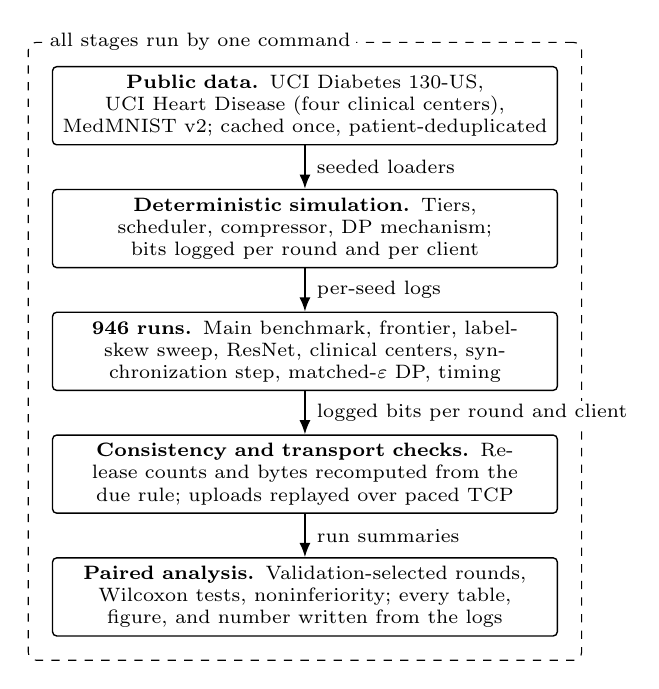
\begin{tikzpicture}[node distance=5.5mm, every node/.style={font=\scriptsize}]
\node[proc, text width=62mm] (d) {\textbf{Public data.} UCI Diabetes 130-US, UCI Heart Disease (four clinical centers), \mbox{MedMNIST v2}; cached once, patient-deduplicated};
\node[proc, text width=62mm, below=of d] (s) {\textbf{Deterministic simulation.} Tiers, scheduler, compressor, DP mechanism; bits logged per round and per client};
\node[proc, text width=62mm, below=of s] (r) {\textbf{946 runs.} Main benchmark, frontier, label-skew sweep, ResNet, clinical centers, synchronization step, matched-$\varepsilon$ DP, timing};
\node[proc, text width=62mm, below=of r] (e) {\textbf{Consistency and transport checks.} Release counts and bytes recomputed from the due rule; uploads replayed over paced TCP};
\node[proc, text width=62mm, below=of e] (a) {\textbf{Paired analysis.} Validation-selected rounds, Wilcoxon tests, noninferiority; every table, figure, and number written from the logs};
\draw[arr] (d) -- node[lab, right=1mm] {seeded loaders} (s);
\draw[arr] (s) -- node[lab, right=1mm] {per-seed logs} (r);
\draw[arr] (r) -- node[lab, right=1mm] {logged bits per round and client} (e);
\draw[arr] (e) -- node[lab, right=1mm] {run summaries} (a);
\begin{scope}[on background layer]
\node[grp, fit=(d)(s)(r)(e)(a), inner sep=3mm, label={[font=\scriptsize, fill=white, inner sep=2pt, anchor=west, xshift=2mm]north west:all stages run by one command}] {};
\end{scope}
\end{tikzpicture}
\caption{Pipeline of the study, from the public data to the reported numbers. All stages are run by one command, which first checks that repeated runs are bit-identical.}
\label{fig:pipeline}
\end{figure}

\subsection{METRICS}
\label{sec:metrics}
We split the patients of each client into training, validation, and test sets (70/10/20\%, patient-grouped) and write $\mathcal V_k$ and $\mathcal T_k$ for the last two. With $\mathrm{AUC}_k^{\mathcal T}(r)$ the AUROC of client $k$'s own model after round $r$ on $\mathcal T_k$, the personalized AUROC and the reported round are
\begin{equation}
\begin{gathered}
A^{\mathcal T}(r)=\frac{\sum_{k}|\mathcal T_k|\,\mathrm{AUC}^{\mathcal T}_k(r)}{\sum_{k}|\mathcal T_k|},\\
\hat r=\min\Big\{\arg\max_{r\le R}A^{\mathcal V}(r)\Big\},
\end{gathered}
\label{eq:metric}
\end{equation}
where $A^{\mathcal V}$ is the same average over the validation splits. A client whose split contains a single class is left out of the corresponding average, identically for every method. The primary metric is $A^{\mathcal T}(\hat r)$; test data are never used to select anything.

The cost that is paired with the primary metric is the upload. With $b_{k,t}$ the bits that client $k$ sends in round $t$, the cumulative upload after round $r$ is
\begin{equation}
B(r)=\frac{1}{8\times10^{6}}\sum_{t=1}^{r}\sum_{k}b_{k,t}\quad\text{(MB)}.
\label{eq:upload}
\end{equation}
We report two readings of (\ref{eq:upload}) and keep them apart throughout. The first, $B(\hat r)$, is the upload needed to obtain the reported model and is the cost that belongs to the primary metric. The second, $B(R)$, is the upload of the whole training budget of $R=60$ rounds, which a deployment without early stopping would send. A full-rate method continues to transmit after its selected round, so $B(R)$ shows a larger saving for sparse schedules than $B(\hat r)$ does, and every statement about a saving names the reading on which it is based.

Secondary metrics are the mean of $A^{\mathcal T}$ over the last 10 rounds, its mean over the rounds of the last 20 that directly follow a synchronization, and its value at $r=R$; the calibration~\cite{vancalster2019}, measured by the expected calibration error (ECE)~\cite{guo2017calibration} and the Brier score~\cite{brier1950} before and after Platt scaling~\cite{platt1999} fitted on $\mathcal V_k$; and the AUROC of the worst client, $\min_k\mathrm{AUC}^{\mathcal T}_k(\hat r)$. Fig.~\ref{fig:pipeline} summarizes the study.

\subsection{PROBLEM STATEMENT}
Given a quota $\rho$ on the payload fraction (\ref{eq:payload}) and, optionally, a cap $\pi$ on the payload of any single round and a privacy budget $(\varepsilon^\star,\delta)$, the scheduler chooses intervals $\mathbf K$ and phases $\boldsymbol\phi$ to solve
\begin{equation}
\max_{\mathbf K,\boldsymbol\phi}\ A^{\mathcal T}(\hat r)\quad\text{s.t.}\quad\Pi_\infty(\mathbf K)\le\rho,\quad\hat P\le\pi,\quad\varepsilon(\mathbf K)\le\varepsilon^\star .
\label{eq:problem}
\end{equation}
We regard a schedule as successful if $A^{\mathcal T}(\hat r)$ is noninferior to that of full-rate personalization and higher than that of the best uniform period at matched bytes, as judged by the rule of Section~\ref{sec:setup}. The objective is not known before training, so Section~\ref{sec:method} optimizes a surrogate. The quantity $\varepsilon(\mathbf K)$ is defined only for a schedule that is fixed before training, because the accountant charges only data-independent releases.

\section{QUOTA-CONSTRAINED MULTI-RATE SCHEDULING}
\label{sec:method}

The scheduler separates four decisions: which parameters are sent (the tiers), when they are sent (per-tier intervals chosen under the quota), how large an upload is (an optional compressor), and how private it is (the DP mechanism and its accountant). Fig.~\ref{fig:arch} shows the architecture.

\begin{figure*}[t]
\centering
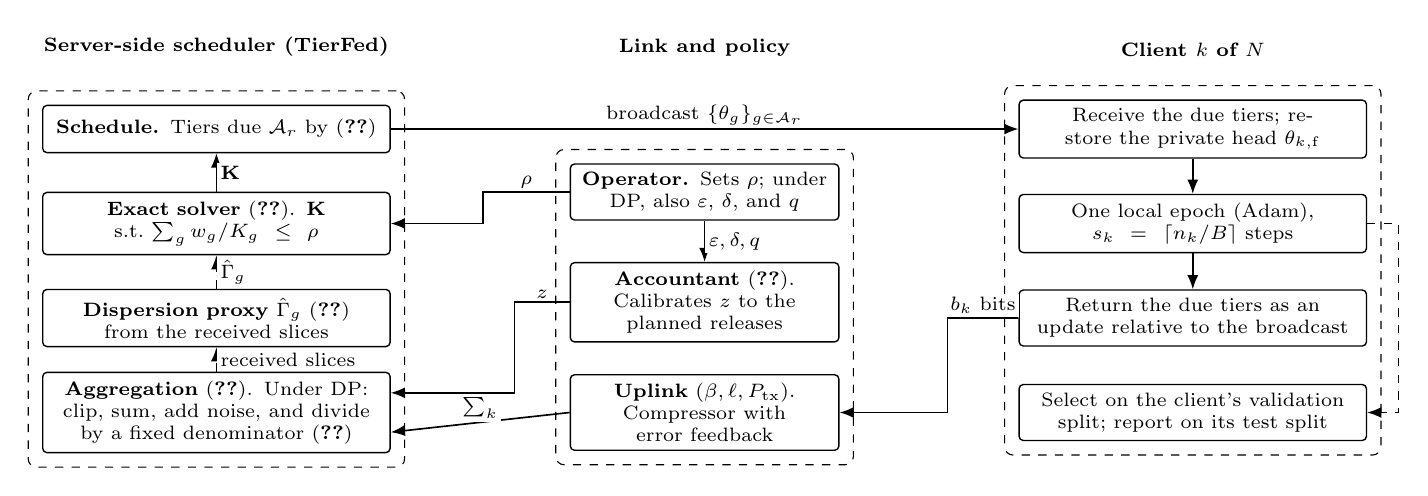
\begin{tikzpicture}[x=1mm,y=1mm]
\node[hdr] at (0,8) {Server-side scheduler (\tierfed{})};
\node[hdr] at (62,8) {Link and policy};
\node[hdr] at (124,8) {Client $k$ of $N$};
% server column
\node[srvbox, text width=42mm] (sched) at (0,0)   {\textbf{Schedule.} Tiers due $\mathcal A_r$ by (\ref{eq:due})};
\node[srvbox, text width=42mm] (solve) at (0,-12) {\textbf{Exact solver} (\ref{eq:ip}). $\mathbf K$ s.t.\ $\sum_g w_g/K_g\le\rho$};
\node[srvbox, text width=42mm] (disp)  at (0,-24) {\textbf{Dispersion proxy} $\Gh_g$ (\ref{eq:gammahat}) from the received slices};
\node[srvbox, text width=42mm] (agg)   at (0,-36) {\textbf{Aggregation} (\ref{eq:agg}). Under DP: clip, sum, add noise, and divide by a fixed denominator (\ref{eq:dp})};
% link column
\node[lnkbox, text width=32mm] (op)   at (62,-8)  {\textbf{Operator.} Sets $\rho$; under DP, also $\varepsilon$, $\delta$, and $q$};
\node[lnkbox, text width=32mm] (acc)  at (62,-22) {\textbf{Accountant} (\ref{eq:rdp}). Calibrates $z$ to the planned releases};
\node[lnkbox, text width=32mm] (link) at (62,-36) {\textbf{Uplink} $(\beta,\ell,P_{\mathrm{tx}})$. Compressor with error feedback};
% client column
\node[stebox, text width=42mm] (bcast) at (124,0)   {Receive the due tiers; restore the private head $\theta_{k,\mathrm f}$};
\node[stebox, text width=42mm] (train) at (124,-12) {One local epoch (Adam), $s_k=\lceil n_k/B\rceil$ steps};
\node[stebox, text width=42mm] (ret)   at (124,-24) {Return the due tiers as an update relative to the broadcast};
\node[stebox, text width=42mm] (eval)  at (124,-36) {Select on the client's validation split; report on its test split};
\begin{scope}[on background layer]
\node[grp, fit=(sched)(solve)(disp)(agg)] {};
\node[grp, fit=(op)(acc)(link)] {};
\node[grp, fit=(bcast)(train)(ret)(eval)] {};
\end{scope}
% data path down the round (solid)
\draw[arr] (sched.east) -- node[lab, above] {broadcast $\{\theta_g\}_{g\in\mathcal A_r}$} (bcast.west);
\draw[arr] (bcast.south) -- (train.north);
\draw[arr] (train.south) -- (ret.north);
\draw[arr] (ret.west) -- ++(-9,0) node[lab, above, pos=0.5] {$b_k$ bits} |- (link.east);
\draw[arr] (link.west) -- node[lab, above] {$\sum_k$} ([yshift=-2.5mm]agg.east);
% policy inputs (solid)
\draw[arr] (op.west) -- ++(-11,0) node[lab, above, pos=0.5] {$\rho$} |- (solve.east);
\draw[arr] (op.south) -- node[lab, right] {$\varepsilon,\delta,q$} (acc.north);
\draw[arr] (acc.west) -- ++(-7,0) node[lab, above, pos=0.5] {$z$} |- ([yshift=2.5mm]agg.east);
% measurements fed back (dashed)
\draw[meas] (agg.north) -- node[lab, right] {received slices} (disp.south);
\draw[meas] (disp.north) -- node[lab, right] {$\Gh_g$} (solve.south);
\draw[arr]  (solve.north) -- node[lab, right] {$\mathbf K$} (sched.south);
\draw[meas] (train.east) -- ++(4,0) |- (eval.east);
\end{tikzpicture}
\caption{Architecture of the scheduler and its environment. Solid arrows carry data and policy inputs, and dashed arrows carry measurements that are fed back. Only the due tiers are broadcast and replaced at the client (\ref{eq:restart}); the other tiers stay at the client and continue to be trained. Under DP, the dashed path from the received slices to the solver is removed, and the schedule is planned before training (Section~\ref{sec:method-privacy}).}
\label{fig:arch}
\end{figure*}

\subsection{DISPERSION MEASUREMENT}
\label{sec:dispersion}
\tierfed{} estimates how strongly the clients disagree on each tier from the uploaded copies of that tier (its slices) that it receives. For tier $g$ with tensors $j\in g$, the estimate is
\begin{equation}
\Gh_g^{(r)}=\frac{\sum_{j\in g}\frac1{|\mathcal S_r|}\sum_{k\in\mathcal S_r}\big\|\theta_{k,j}^{(r,s_k)}-\bar\theta_j^{(r)}\big\|_2^2}{\sum_{j\in g}\big\|\bar\theta_j^{(r)}\big\|_2^2+\xi_0},
\label{eq:gammahat}
\end{equation}
where $\bar\theta_j^{(r)}$ is the unweighted mean of the received tensors and $\xi_0=10^{-12}$. The ratio is scale-free, which makes tiers of different magnitudes comparable. It is available only for the tiers received in round $r$, and the last value is carried forward for the others.

Under the restart step, the received slices are one local epoch away from a common value, so $\Gh_g$ does not depend on the interval that preceded the upload, and the scheduler does not measure the effect of its own earlier decisions. The logs confirm this. For uniform periods $K$ from 1 to 8 on the main benchmark, the mean of $\Gh_g$ over the synchronization rounds after warm-up lies between $4.59\times10^{-3}$ and $5.93\times10^{-3}$ for the slow tier and between $6.93\times10^{-3}$ and $7.71\times10^{-3}$ for the medium tier (supplement, Table~S-IV). Under the carry-over step, the same quantity grows with the interval: it is larger than under the restart step by factors of 7.5 and 5.3 for the two tiers at $K=4$ and of 26.9 and 11.9 at $K=8$.

\subsection{COST OF AN INTERVAL, PROGRAM, AND CLOSED FORM}
\label{sec:program}
\emph{Assumptions.} We analyze the shared tiers with the private heads held fixed and assume local SGD with step size $\eta$ in place of Adam, the same number $s$ of local steps at every client, and equal aggregation weights $1/N$. We also assume that each $F_k$ is block separable, $F_k(\theta)=\sum_gF_{k,g}(\theta_g)$, with $L$-smooth blocks, so that the gradient of a tier does not depend on the other tiers. This assumption removes the coupling between tiers and is the main idealization. Stochastic gradients are unbiased with variance at most $\sigma_g^2$ on tier $g$; the heterogeneity of tier $g$ is bounded, $\frac1N\sum_k\|\nabla_gF_k(\theta)-\nabla_gF(\theta)\|^2\le\Gamma_g$; and $F_g=\frac1N\sum_kF_{k,g}$ is bounded below by $F_g^\star$~\cite{wang2021coop}. The experiments depart from these assumptions in that they use Adam, $s_k=\lceil n_k/B\rceil$ steps, sample weights, and a coupled network; with unequal $s_k$, plain averaging converges toward a reweighted objective~\cite{wang2020fednova}. The two propositions describe the idealized system. We use them to motivate the schedule, not to predict accuracy.

\begin{proposition}[Cost of an interval under the restart step]
\label{prop:bound}
Let tier $g$ be synchronized every $K_g$ rounds by (\ref{eq:restart})--(\ref{eq:adopt}). There are absolute constants $c_0,c_1,c_2$ such that the following holds for $\eta\le c_0/(LK_{\max}s)$, where $K_{\max}$ is the largest interval that the scheduler may assign.

\noindent(a) \emph{Client copies.} After $m\ge1$ local epochs from a common value of tier $g$, with $\bar\theta_g=\frac1N\sum_k\theta_{k,g}$,
\begin{equation}
\frac1N\sum_{k=1}^N\mathbb E\big\|\theta_{k,g}-\bar\theta_g\big\|^2\le c_2\,\eta^2s^2m^2\big(\Gamma_g+\sigma_g^2\big),
\label{eq:drift}
\end{equation}
and $m\le\max(1,K_g-1)\le K_g$ at every point of the schedule.

\noindent(b) \emph{Server copy.} Let $r_1<\dots<r_{J_g}$ be the rounds up to $R$ in which tier $g$ is due, and $D_g=F_g(\theta_g^{(1)})-F_g^\star$. Then
\begin{align}
\min_{1\le j\le J_g}\mathbb E\big\|\nabla_gF(\theta^{(r_j)})\big\|^2
&\le \frac{c_1D_g}{\eta sJ_g}+c_1\eta L\,\frac{\sigma_g^2}{N}\notag\\
&\quad+c_2\,\eta^2L^2s^2\big(\Gamma_g+\sigma_g^2\big).
\label{eq:bound}
\end{align}
\end{proposition}
The proof is given in the supplement (Section~S1). Part (a) is the drift lemma of local SGD~\cite{stich2019,khaled2020} applied to one tier. Part (b) holds because, under block separability, the steps that a client takes on a tier between two synchronizations of that tier never enter the server copy, so the synchronizations of tier $g$ form a sequence of $J_g$ rounds of federated averaging with $s$ local steps~\cite{wang2020fednova,karimireddy2020}. The variance in the second term of (\ref{eq:bound}) is divided by $N$ because every step of the averaged model combines one stochastic gradient from each client. These $N$ gradients are independent, each has a variance of at most $\sigma_g^2$, and their average with equal weights therefore has a variance of at most $\sigma_g^2/N$, which is the linear speedup of local SGD in the number of clients. With the sample weights $p_k$ of (\ref{eq:agg}), the factor $1/N$ becomes $\sum_kp_k^2=1/N_{\mathrm{eff}}$. On the main benchmark, $\sum_kp_k^2=0.085$, which corresponds to $N_{\mathrm{eff}}=11.8$ for $N=20$, and at the clinical centers, $N_{\mathrm{eff}}=3.6$ for $N=4$.

Under the restart step, an interval therefore has two costs. By (\ref{eq:bound}), the server copy of tier $g$ receives $J_g\approx T_w+(R-T_w)/K_g$ aggregation rounds instead of $R$, so the first term grows with $K_g$, whereas the last term does not depend on $K_g$. By (\ref{eq:drift}), the clients' own copies, which are the models that are evaluated, drift apart between synchronizations by an amount that grows as $K_g^2$. Under the carry-over step, the two costs merge into the bound of local SGD with period $K_gs$~\cite{wang2021coop}: the $K_g$ local epochs enter the average, $J_g$ is replaced by $R$, and the last term of (\ref{eq:bound}) becomes $c_2\eta^2L^2s^2K_g^2(\Gamma_g+\sigma_g^2)$. In both cases, $K_g^2(\Gamma_g+\sigma_g^2)$ measures what a long interval costs on tier $g$, and it is small only for a tier on which the clients agree.

\emph{Program.} Given a quota $\rho$, the scheduler solves
\begin{equation}
\mathbf K^\star=\arg\min_{K_g\in\{1,\dots,K_{\max}\}}\sum_{g\in\mathcal G_{\mathrm{sh}}}K_g^2\,\Gh_g\ \ \text{s.t.}\ \sum_{g\in\mathcal G_{\mathrm{sh}}}\frac{w_g}{K_g}\le\rho .
\label{eq:ip}
\end{equation}
The objective is the right-hand side of (\ref{eq:drift}) with $m$ replaced by its upper bound $K_g$, summed over the shared tiers, with the measured $\Gh_g$ in place of $\Gamma_g+\sigma_g^2$; the factor $c_2\eta^2s^2$ is common to the tiers and does not change the minimizer. The measured dispersion $\Gh_g$ is a proxy for $\Gamma_g+\sigma_g^2$ and not an estimate of it. Its numerator is the dispersion after one local epoch, in which the noise and the heterogeneity enter with different powers of $s$, and its denominator is the squared norm of the tier, which differs between tiers. Nor does the program contain the server-side cost of (\ref{eq:bound}). It is thus a heuristic surrogate, and every statement below about (\ref{eq:ip}) concerns this surrogate. With the head private, $\mathcal G_{\mathrm{sh}}=\{\mathrm s,\mathrm m\}$, and with $K_{\max}=8$, the program has 64 candidates and is solved by enumeration, with ties broken in favor of the denser schedule.

\begin{proposition}[Closed form and the value of differentiation]
\label{prop:cuberoot}
Let $\Gamma_g>0$, $w_g>0$, and $\sum_gw_g=1$, let $\Gamma_g$ replace $\Gh_g$ in (\ref{eq:ip}), and let $K_g$ be relaxed to the positive reals. Then (\ref{eq:ip}) has the unique minimizer
\begin{equation}
K_g^\star=\Big(\frac{w_g}{\Gamma_g}\Big)^{1/3}\frac{S}{\rho},\qquad S=\sum_hw_h^{2/3}\Gamma_h^{1/3},
\label{eq:cuberoot}
\end{equation}
with value $J^\star=S^3/\rho^2$. The uniform period $K=1/\rho$ costs $J_{\mathrm u}=\sum_g\Gamma_g/\rho^2$, and
\begin{equation}
\Psi=1-\frac{J^\star}{J_{\mathrm u}}=1-\frac{S^3}{\sum_g\Gamma_g}\in[0,1),
\label{eq:psi}
\end{equation}
with $\Psi=0$ if and only if $w_g/\Gamma_g$ is the same for all tiers. When $1/\rho$ is an integer, no integer schedule lowers the objective of (\ref{eq:ip}) below that of the uniform period by more than the fraction $\Psi$.
\end{proposition}
The proof (supplement, Section~S1) uses the Karush--Kuhn--Tucker conditions of the convex program, H\"older's inequality with exponents $3/2$ and $3$ for $\Psi\ge0$, and the integer feasibility of $K=1/\rho$. We use two properties of the closed form in the evaluation. First, the ratio of two intervals, $K_a/K_b=\big(w_a\Gamma_b/(w_b\Gamma_a)\big)^{1/3}$, compresses differences between tiers: a factor of eight in the ratio of payload to dispersion is needed for a factor of two in the interval, so tiers with similar ratios receive the same interval after rounding. Second, the proposition holds for any positive values of $\Gamma_g$ and therefore applies exactly to (\ref{eq:ip}) as stated, with the measured $\Gh_g$. The quantity $\Psi$ is invariant to a factor common to all tiers. Evaluated on $\Gh_g$ at the end of warm-up, it states, before any sparse round has taken place, by how much a per-tier schedule can lower the surrogate below that of a uniform one. It does not state how much accuracy such a reduction is worth.

\subsection{SCHEDULE RULE, PHASES, AND THE QUOTA}
Rounds are indexed $r=1,\dots,R$. The first $T_w$ rounds synchronize every shared tier, and thereafter tier $g$ is due according to
\begin{equation}
\mathcal A_r=\begin{cases}\mathcal G_{\mathrm{sh}}, & r\le T_w,\\ \{g:\ (r-T_w-\phi_g)\bmod K_g=0\}, & r>T_w,\end{cases}
\label{eq:due}
\end{equation}
with phase $\phi_g=0$ unless the tiers are staggered. The fixed periods, the DP planner, and the accountant all use this rule, and the consistency check of Section~\ref{sec:results-check} recomputes every release from it. Adaptive \tierfed{} sends tier $g$ when at least $K_g$ rounds have passed since its last synchronization, which coincides with (\ref{eq:due}) whenever $\mathbf K$ is constant after warm-up. We set $T_w=5$ and $K_{\max}=8$ throughout. Fig.~\ref{fig:round} shows one round at the server.

\emph{Phases and the peak.} A quota on the mean does not bound the payload $P_r$ of a single round, because tiers with aligned phases are due together and then send the full shared payload. Over a horizon of at least $\mathrm{lcm}(K_a,K_b)$ rounds after warm-up, two tiers with phases $\phi_a$ and $\phi_b$ are never due in the same round if and only if $\phi_a-\phi_b\not\equiv0\pmod{\gcd(K_a,K_b)}$ (supplement, Section~S1). With $\gcd(K_a,K_b)\ge2$, the offset $\lfloor\gcd(K_a,K_b)/2\rfloor$ separates them and bounds the peak after warm-up by $\max_gw_g$ at the same long-run payload fraction $\Pi_\infty$; over a finite horizon, $\Pi_R$ can differ slightly, because the phase changes which synchronizations fall inside it. With coprime intervals, no phase separates the tiers. The staggered variant adds the constraint $\max_{r>T_w}P_r\le\pi$ to (\ref{eq:ip}) and checks it over one hyperperiod $\mathrm{lcm}(\mathbf K)$. The warm-up rounds still send the whole payload, and their uploads can be sent with 8-bit quantization to lower their peak as well.

\emph{The quota.} Solving (\ref{eq:ip}) with $\rho$ bounds $\Pi_\infty$ of (\ref{eq:payload}) and not the realized $\Pi_R$: a warm-up of $T_w$ rounds at payload fraction $c_w$ adds $T_w(c_w-\Pi_\infty)/R$ to the realized fraction. A quota over all rounds is met by solving with $\rho'=(\rho R-c_wT_w)/(R-T_w)$. We report both forms and read the realized $\Pi_R$ from the logs.

\begin{figure}[t]
\centering
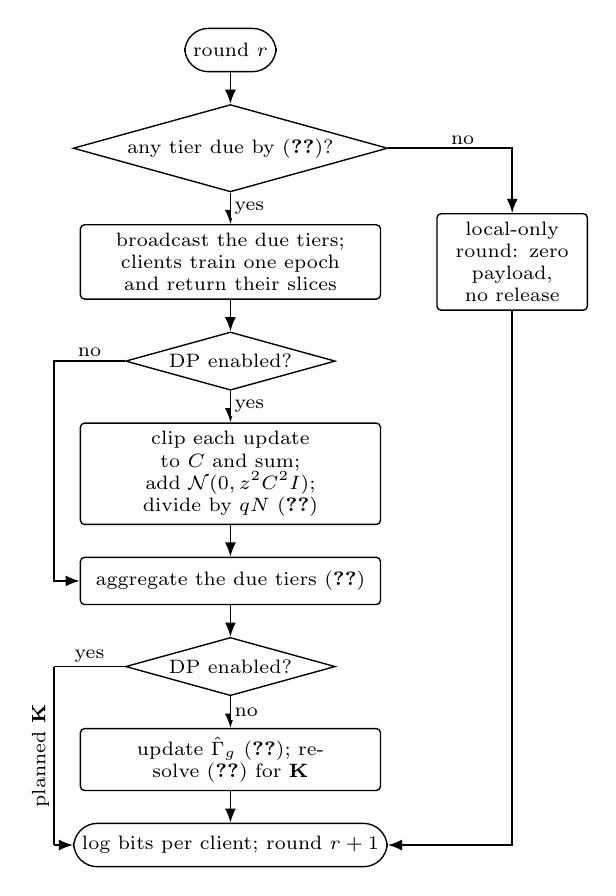
\begin{tikzpicture}[node distance=4mm and 6mm, every node/.style={font=\scriptsize}]
\node[term] (start) {round $r$};
\node[dec, below=of start] (due) {any tier due by (\ref{eq:due})?};
\node[proc, text width=36mm, below=of due] (bc) {broadcast the due tiers; clients train one epoch and return their slices};
\node[dec, below=of bc] (dp) {DP enabled?};
\node[proc, text width=36mm, below=of dp] (priv) {clip each update to $C$ and sum;\\ add $\mathcal N(0,z^2C^2I)$;\\ divide by $qN$ (\ref{eq:dp})};
\node[proc, text width=36mm, below=of priv] (ag) {aggregate the due tiers (\ref{eq:agg})};
\node[dec, below=of ag] (dp2) {DP enabled?};
\node[proc, text width=36mm, below=of dp2] (upd) {update $\Gh_g$ (\ref{eq:gammahat}); re-solve (\ref{eq:ip}) for $\mathbf K$};
\node[term, below=of upd] (next) {log bits per client; round $r+1$};
\node[proc, text width=17mm, right=7mm of bc] (local) {local-only round: zero payload, no release};
\draw[arr] (start) -- (due);
\draw[arr] (due) -- node[lab, right] {yes} (bc);
\draw[arr] (due.east) -| node[lab, above, pos=0.3] {no} (local);
\draw[arr] (local.south) |- (next.east);
\draw[arr] (bc) -- (dp);
\draw[arr] (dp) -- node[lab, right] {yes} (priv);
\draw[arr] (dp.west) -- ++(-9mm,0) node[lab, above, pos=0.5] {no} |- (ag.west);
\draw[arr] (priv) -- (ag);
\draw[arr] (ag) -- (dp2);
\draw[arr] (dp2) -- node[lab, right] {no} (upd);
\coordinate (k1) at ($(dp2.west)+(-9mm,0)$);
\coordinate (k2) at (k1 |- next.west);
\draw[line width=0.6pt] (dp2.west) -- node[lab, above] {yes} (k1);
\draw[line width=0.6pt] (k1) -- node[midway, rotate=90, anchor=south, font=\scriptsize, inner sep=1.5pt] {planned $\mathbf K$} (k2);
\draw[arr] (k2) -- (next.west);
\draw[arr] (upd) -- (next);
\end{tikzpicture}
\caption{Flow of one round at the server. In a local-only round, the clients still train their own copies. Under DP, the schedule is fixed before training, and the scheduler never receives the private slices; the simulator logs their dispersion and the clipped share only as diagnostics, which are outside the accounted release.}
\label{fig:round}
\end{figure}

\emph{Compression.} An optional compressor acts on each client's update relative to the broadcast, with error feedback. It emits a fraction $\kappa\in(0,1]$ of the float32 bits, and the bits that it emits are the bits that are counted.

\subsection{PRIVACY: THREAT MODEL, MECHANISM, AND ELIGIBLE SCHEDULES}
\label{sec:method-privacy}
\emph{Threat model.} Clients send their updates over Transport Layer Security to an aggregator that is trusted to apply the mechanism and sees the raw updates, as in central DP-FedAvg~\cite{mcmahan2018dp}. Central DP protects the data of each client against those who receive the released aggregates, including the other clients. A passive network observer cannot read the payloads but sees when each client transmits and how many bytes it sends, which is exactly the schedule. A schedule that depends on client data can therefore leak information even when every payload is encrypted. Secure aggregation with distributed noise~\cite{kairouz2021ddg} would remove the need to trust the aggregator but not this metadata. Poisoning is outside the scope of this article.

\emph{Mechanism.} In each round, every client joins the cohort $\mathcal S_r$ independently with probability $q$. Full participation, $q=1$, is the primary cross-silo setting, and we examine $q<1$ as a sensitivity analysis. The server clips the update $\Delta_k=\theta_k^{(r,s_k)}-\theta^{(r)}$ of every participating client on the due tiers and adds noise to the sum before dividing by the \emph{fixed} expected cohort size,
\begin{equation}
\tilde\Delta=\frac1{qN}\Big(\sum_{k\in\mathcal S_r}\Delta_k\min\big(1,\tfrac{C}{\|\Delta_k\|_2}\big)+\mathcal N(0,z^2C^2I)\Big),
\label{eq:dp}
\end{equation}
which is the fixed-denominator estimator of DP-FedAvg~\cite{mcmahan2018dp} with clipping norm $C$ and noise multiplier $z$. Adding or removing one client changes the sum by at most $C$ in $\ell_2$ norm, and the denominator reveals nothing about the realized cohort; a planned release whose cohort is empty still adds noise. Because of the restart step, $\Delta_k$ is the result of one local epoch for every schedule, so the clipping norm $C$ has the same meaning for all of them. The server applies the mechanism to every method in the same way.

\emph{Accountant.} Over the $R_{\mathrm{tx}}$ planned releases, the R\'enyi DP of the Poisson-subsampled Gaussian mechanism is composed over a grid of orders $\alpha$~\cite{mironov2019sgm},
\begin{align}
\varepsilon_\alpha&=\frac{R_{\mathrm{tx}}}{\alpha-1}\log\sum_{k=0}^{\alpha}\binom{\alpha}{k}(1-q)^{\alpha-k}q^ke^{\frac{k^2-k}{2z^2}},\notag\\
\varepsilon&=\min_\alpha\Big\{\varepsilon_\alpha+\frac{\log(1/\delta)}{\alpha-1}\Big\},
\label{eq:rdp}
\end{align}
with $\delta=10^{-5}$; for $q=1$, this reduces to $R_{\mathrm{tx}}\alpha/(2z^2)$~\cite{mironov2017}. We check the implementation against the TensorFlow Privacy reference (supplement, Section~S2); for $q=1$, our implementation evaluates the closed form directly. At $q=1$, the exact privacy of $R_{\mathrm{tx}}$ Gaussian releases is $\mu$-Gaussian DP with $\mu=\sqrt{R_{\mathrm{tx}}}/z$~\cite{dong2022gdp}, whose $(\varepsilon,\delta)$ curve is that of the analytic Gaussian mechanism~\cite{balle2018}. This exact accountant and (\ref{eq:rdp}) both depend on $R_{\mathrm{tx}}$ only through $R_{\mathrm{tx}}/z^2$, so the exact one would lower the noise multiplier of every method by the same proportion, between 13\% and 24\% for $\varepsilon^\star$ from 8 to 1 (supplement, Section~S2). The comparison at matched $\varepsilon$ is unaffected by the choice of accountant, and every reported $\varepsilon$ is an upper bound. We calibrate the multiplier $z$ to the release count of each method by bisection on (\ref{eq:rdp}).

\emph{Which schedules are covered.} The accountant covers a release only if the decision to release does not depend on the private data. This holds for FedAvg, FedProx, FedPer, local training, a fixed period, and the planner described below, whose release rounds are fixed before training. It does not hold for adaptive \tierfed{}, AdaComm, LAG, or the FedLAMA-style rule~\cite{lee2023fedlama} of Section~\ref{sec:setup}, whose schedules are functions of client updates or losses, and the released code refuses to run these under DP unless an explicit override is set; the override is kept only to reproduce earlier logs that are not reported here. Privacy filters and odometers~\cite{rogers2016odometer} and the sparse vector technique~\cite{lyu2017svt} charge for data-dependent release decisions, whereas the adaptive FL schedulers listed above make such decisions without charging for them. DP follow-the-regularized-leader~\cite{kairouz2021ftrl} and matrix-factorization mechanisms~\cite{choquette2023banded} are suited to full participation but also require data-independent release rounds, and we do not evaluate them here.

\emph{Planning under a privacy budget (\tierfed{}-DP).} A planner that respects the accountant chooses $\mathbf K$ before training from public quantities only: $(\varepsilon^\star,\delta)$, $q$, $R$, $T_w$, $w_g$, and $\rho$. For each candidate, it computes the release set of (\ref{eq:due}) and the smallest $z(\mathbf K)$ that keeps these releases $(\varepsilon^\star,\delta)$-DP, and it minimizes
\begin{equation}
J(\mathbf K)=\frac{\sum_g w_gK_g^2}{K_{\max}^2}+\lambda\,\frac{\sum_{r}P_r(\mathbf K)\,z(\mathbf K)^2}{\sum_{r}P_r(\mathbf 1)\,z(\mathbf 1)^2}
\label{eq:jdp}
\end{equation}
over the candidates whose realized payload fraction $\Pi_R$, warm-up included, is within the quota. The first term is the drift cost of (\ref{eq:ip}) under a flat prior $\Gamma_g\propto w_g$, and the second, weighted by $\lambda\ge0$, is the injected noise energy; each is normalized by its largest value. Fewer releases need less noise but allow more drift. Under the flat prior, Proposition~\ref{prop:cuberoot} gives $\Psi=0$, so the relaxed minimizer of the first term is a uniform period. The integer planner is not restricted to equal intervals, however. Evaluated on a grid of 35 combinations of the noise weight $\lambda$ and the quota (supplement, Table~S-III), it returns equal intervals in 31 of them, including all those in which the quota does not bind. In the remaining 4, all at $\rho=0.25$, where the warm-up rounds make $(4,4)$ infeasible, it returns the unequal pair $(5,6)$. The choice does not depend on $\varepsilon^\star$. In the DP experiments of this article, which use $\rho=1$ and $\lambda=1$, the planner selects $(3,3)$ in every seed. We evaluate it as an ablation of planning under a budget and do not claim it as a contribution.

\section{EXPERIMENTAL SETUP}
\label{sec:setup}
We run every method under the protocol of Section~\ref{sec:system} on the same seeds and data splits, and we read every number from the logs. Table~\ref{tab:setup} summarizes the configuration.


\emph{Experiment families.} The main protocol comprises 946 runs, which are listed by family in the supplement (Table~S-V): the main comparison on the specialty groups and at the clinical centers; the accuracy--upload frontier with the communication parameter of every method swept; the label-skew sweep and the ResNet-backbone runs, which examine the regimes to which Proposition~\ref{prop:cuberoot} points; the round-sparse schedules with the carry-over step of Section~\ref{sec:federation}; and the matched-$\varepsilon$, timing, and peak-aware runs. Additional experiments that were read at the final round without a validation split are reported in Section~S9 of the supplement and are identified there as such.

\emph{Baselines and bounds.} The full-rate methods are FedAvg~\cite{mcmahan2017}, FedProx~\cite{li2020fedprox}, and FedPer~\cite{arivazhagan2019}, the last of which is the reference for the noninferiority tests. The round-sparse methods are AdaComm~\cite{wang2019adacomm}, LAG~\cite{chen2018lag}, a FedLAMA-style per-layer interval rule reimplemented from its published description~\cite{lee2023fedlama}, and fixed periods on (\ref{eq:due}) with the private head and the warm-up of \tierfed{}. We run LAG with the sample weights of (\ref{eq:agg}) and, as a variant, with equal client weights. Unless another value is stated, AdaComm starts from an initial period of 8, its period is capped at the larger of 8 and the initial period, and LAG uses the threshold $\xi=1$. All round-sparse methods run under the protocol of Section~\ref{sec:federation}, restart step included, so that the comparison isolates the schedule. As published, AdaComm and the fixed local period upload the result of all local steps since the last synchronization; this corresponds to the carry-over step, which we evaluate in Section~\ref{sec:results-sync}. Three references bracket the attainable accuracy: local training without communication, a centralized multilayer perceptron (MLP) trained on the pooled training splits of all clients for the same number of passes, and histogram-based gradient boosting (the scikit-learn implementation, which is modeled on LightGBM~\cite{ke2017lightgbm}). All three are scored on the same per-client test splits, with the round, epoch, or iteration chosen on the validation split. SCAFFOLD~\cite{karimireddy2020}, whose control variates are defined for SGD, is reported with an SGD local solver in the supplement.

\emph{Differential privacy.} We run FedPer, the fixed periods $K=4$ and $K=8$, one-shot federation (no warm-up and a single release in round $R$, after a data-independent broadcast of the initial model), and the planner at $\varepsilon^\star=4$, $\delta=10^{-5}$, $q=1$, and $C=1$, each with $z$ calibrated to its own release count. Local training is the reference with $\varepsilon=0$ on the same splits. Sweeps with $q<1$ over $\varepsilon^\star\in\{1,2,4,8\}$ for 20 and 100 clients are reported in the supplement.

\emph{Timing side channel.} The timing experiment compares two worlds. In the shifted world, each label of one target client is flipped with probability 0.5; in the clean world, none is flipped. A passive observer sees which rounds carry traffic and how many bytes each client sends, and summarizes a run by one of four observables $o$: the number of rounds with traffic, the number of rounds in which the target transmits, the bytes of the target, or the bytes of all clients. We measure the power of the observer by the Mann--Whitney area under the curve (AUC) over the $n_1$ shifted and $n_0$ clean runs,
\begin{equation}
\mathrm{AUC}=\frac1{n_1n_0}\sum_{i=1}^{n_1}\sum_{j=1}^{n_0}\Big(\mathbb 1\big[o^{(1)}_i>o^{(0)}_j\big]+\tfrac12\,\mathbb 1\big[o^{(1)}_i=o^{(0)}_j\big]\Big),
\label{eq:auc}
\end{equation}
where $o^{(1)}_i$ and $o^{(0)}_j$ are the values of the observable in the shifted and the clean runs; the AUC equals 0.5 when the schedule reveals nothing. We assess its significance by a permutation test whose statistic is the largest value of $|\mathrm{AUC}-0.5|$ over the four observables; the null distribution is obtained from 10,000 random reassignments of the runs to the two worlds, which accounts for the choice among observables. We report a schedule as leaking when $|\mathrm{AUC}-0.5|\ge0.25$ on at least one observable and the permutation $p$-value is below 0.05.

\emph{Statistics.} All comparisons are paired across seeds. Before the runs, we fixed in the code the metric, the byte tolerance, and the relevance threshold used below, as well as two primary contrasts: \tierfed{} against FedPer, and \tierfed{} against the best uniform period at matched bytes. With $\mathcal U$ denoting the uniform periods run in a setting, $B_K$ the mean upload $B(R)$ of period $K$, $B_{\mathrm{TF}}$ that of \tierfed{}, and $\bar A^{\mathcal V}_K$ the mean validation AUROC at $\hat r$, the best uniform period and the gain over it are
\begin{equation}
\begin{gathered}
K_{\mathrm u}=\arg\max_{K\in\mathcal U:\,B_K\le1.05\,B_{\mathrm{TF}}}\bar A^{\mathcal V}_K,\\
\Delta_{\mathrm u}=\frac1M\sum_{i=1}^{M}\big(A^{\mathcal T}_{\mathrm{TF},i}-A^{\mathcal T}_{K_{\mathrm u},i}\big),
\end{gathered}
\label{eq:gate}
\end{equation}
where $A^{\mathcal T}_{\mathrm{TF},i}$ and $A^{\mathcal T}_{K_{\mathrm u},i}$ are the values of $A^{\mathcal T}(\hat r)$ of \tierfed{} and of the period $K_{\mathrm u}$ in seed $i$, and the mean is taken over the $M$ seeds that \tierfed{} and that period share. Every other comparison is exploratory. Tests are two-sided Wilcoxon signed-rank tests, and the 95\% confidence intervals (CIs), referred to below as intervals where no confusion with the synchronization intervals $K_g$ can arise, are percentile bootstrap intervals over seeds with 10,000 resamples. We first specified the second contrast with a Holm-corrected $p<0.05$, which the smallest families cannot reach by construction, and so we judge $\Delta_{\mathrm u}$ by its interval instead: a setting counts as a gain only if the 95\% interval excludes zero and $\Delta_{\mathrm u}\ge0.005$ AUROC. No setting meets either the Holm-corrected criterion or the interval criterion. We do not call a difference below 0.005 AUROC relevant, whatever its $p$-value. Noninferiority to FedPer is tested one-sided,
\begin{equation}
H_0:\ \mathbb E[d]\le-\Delta_{\mathrm{NI}},\qquad d=A^{\mathcal T}_{\text{method}}(\hat r)-A^{\mathcal T}_{\text{FedPer}}(\hat r),
\label{eq:ni}
\end{equation}
by the signed-rank test on $d+\Delta_{\mathrm{NI}}$ with $\Delta_{\mathrm{NI}}=0.01$ and, as a sensitivity margin, 0.005. Repeated runs are bit-identical on one machine. On a second machine, every data-independent schedule sends the same bytes, but the AUROC of a single run can change by up to 0.0893 (Section~\ref{sec:results-check}), so we compute every comparison within one machine.

\section{RESULTS}
\label{sec:results}

This section reports the checks of the protocol, the main comparison on both benchmarks, the settings in which a per-tier schedule could be expected to help, the effect of the synchronization step, the cost on constrained links, and privacy. Unless stated otherwise, values are means over seeds on the readmission data with the MLP and the specialty groups, and $p$-values are from paired Wilcoxon tests.

\subsection{PROTOCOL CHECKS}
\label{sec:results-check}
The consistency check finds no mismatches. From the stated rules, it recomputes the transmitting rounds of every data-independent schedule, the bits of every uncompressed round with full participation, and the releases charged by the accountant, over all 2,760 logs of the released repository. These comprise the 946 runs of the main protocol, one single-seed check, and 1,813 runs of the additional experiments (supplement, Section~S9) and of earlier experiments that are not reported. The 1,249 schedule checks, 1,144 byte checks, and 250 accountant checks all agree.

We performed all runs of the main protocol on one Linux machine and repeated 136 of the label-skew and timing runs on a Windows laptop. Every data-independent schedule sends the same bytes in every round on both machines, and so do 31 of the 44 adaptive runs; the others differ by up to 2.9\%, because their decisions depend on floating-point values computed from client data. The AUROC at the selected round changes by a median of 0.0003 and by at most 0.0893. The maximum occurs under strong label skew, where the validation curve is flat and a small numerical difference selects another round; the selected round differs in 39 of the 136 runs. The outcome of the second primary contrast in the label-skew settings is the same on both machines, and for each of the three schedules that were repeated (Fixed $(4,4)$, \tierfed{}, and LAG with $\xi=2000$), the observer AUC of the timing experiment lies on the same side of 0.75.

Because the selected round can move in this way, we repeat both primary contrasts under two other rules: the first maximum of the trailing three-round mean of $A^{\mathcal V}$ (the smoothed rule), and the mean of $A^{\mathcal T}$ over the last 10 rounds, which involves no selection (supplement, Section~S3). Under none of the three rules is \tierfed{} ahead of the best uniform period by 0.005 AUROC with an interval above zero in any setting. Its agreement with FedPer is less stable. Under the smoothed rule, it is below FedPer by more than 0.005, with an interval below zero, in two of the seven settings (Dirichlet $\alpha=10$: \ensuremath{-}0.0125 [\ensuremath{-}0.0168, \ensuremath{-}0.0090]; ResNet backbone: \ensuremath{-}0.0055 [\ensuremath{-}0.0088, \ensuremath{-}0.0025]); at the clinical centers, the upper limit of the interval is zero to four decimal places (supplement, Table~S-I). These shortfalls arise because the first-maximum rule of (\ref{eq:metric}) can select the peak that follows a synchronization.

\begin{table*}[t]
\caption{Comparison of the Methods on the 20 Specialty Groups}
\label{tab:main}
\centering\footnotesize\setlength{\tabcolsep}{3pt}
\fit{\begin{tabular}{@{}lcccccccccc@{}}
\toprule
Method & AUROC at $\hat r$ [95\% CI] & MB to $\hat r$ & MB, 60 rounds & Last 10 & Phase & Fine-tuned & ECE raw/Platt & Worst group & $\Delta$ FedPer & $p$\\
\midrule
Local only & 0.6145 [0.6091, 0.6203] & 0.0 & 0.0 & 0.5557 & 0.5564 & 0.5548 & 0.363/0.023 & 0.431 & \ensuremath{-}0.0239 & 0.002\\
FedAvg & 0.6391 [0.6341, 0.6447] & 50.6 & 218.4 & 0.6230 & 0.6252 & 0.6069 & 0.365/0.024 & 0.468 & \ensuremath{+}0.0006 & 0.064\\
FedProx & 0.6391 [0.6349, 0.6439] & 77.9 & 218.4 & 0.6283 & 0.6306 & 0.6108 & 0.361/0.025 & 0.488 & \ensuremath{+}0.0006 & 0.432\\
FedPer & 0.6385 [0.6337, 0.6437] & 63.2 & 217.8 & 0.6261 & 0.6279 & 0.6083 & 0.367/0.024 & 0.468 & -- & --\\
FedLAMA-style & 0.6396 [0.6344, 0.6457] & 49.4 & 154.1 & 0.6314 & 0.6329 & 0.6119 & 0.363/0.024 & 0.476 & \ensuremath{+}0.0011 & 0.131\\
AdaComm & 0.6329 [0.6273, 0.6391] & 27.7 & 29.1 & 0.6302 & 0.6300 & 0.6234 & 0.363/0.023 & 0.463 & \ensuremath{-}0.0056 & 0.004\\
LAG, equal weights & 0.6373 [0.6328, 0.6419] & 116.9 & 218.4 & 0.6344 & 0.6350 & 0.6218 & 0.362/0.024 & 0.480 & \ensuremath{-}0.0012 & 0.492\\
LAG & 0.6395 [0.6341, 0.6457] & 44.4 & 218.4 & 0.6237 & 0.6259 & 0.6079 & 0.366/0.024 & 0.470 & \ensuremath{+}0.0011 & 0.064\\
Fixed (8,8) & 0.6372 [0.6318, 0.6438] & 35.9 & 39.9 & 0.6280 & 0.6379 & 0.6003 & 0.363/0.024 & 0.457 & \ensuremath{-}0.0013 & 0.275\\
\tierfed{} $\equiv$ Fixed (4,4) & 0.6377 [0.6328, 0.6439] & 45.7 & 65.3 & 0.6346 & 0.6396 & 0.6122 & 0.361/0.024 & 0.463 & \ensuremath{-}0.0007 & 0.557\\
\tierfed{}, staggered $\equiv$ Staggered (4,4) & 0.6353 [0.6309, 0.6400] & 40.2 & 67.0 & 0.6289 & 0.6327 & 0.6112 & 0.359/0.024 & 0.447 & \ensuremath{-}0.0032 & 0.049\\
\midrule
Centralized MLP & 0.6435 [0.6373, 0.6505] & -- & -- & 0.5936 & -- & -- & 0.363/-- & -- & \ensuremath{+}0.0050 & 0.004\\
Gradient boosting & 0.6413 [0.6348, 0.6490] & -- & -- & 0.6272 & -- & -- & 0.019/-- & -- & \ensuremath{+}0.0029 & 0.160\\
\bottomrule
\end{tabular}}
\tabnote{MLP, means over 10 seeds. AUROC at $\hat r$: personalized test AUROC at the validation-selected round with its bootstrap 95\% interval. MB to $\hat r$ and MB, 60 rounds: the readings $B(\hat r)$ and $B(R)$ of the upload (\ref{eq:upload}). Last 10 and Phase: mean AUROC over the last 10 rounds and over the post-synchronization rounds of the last 20. Fine-tuned: final model after three further local epochs. For the two reference bounds below the rule, Last 10 is the mean over the last 10 training epochs (centralized MLP) or over the last 10 evaluations, made every 10 boosting iterations (gradient boosting). ECE: without and with Platt scaling. Worst group: lowest AUROC of a group at $\hat r$. $\Delta$ FedPer and $p$: paired difference from FedPer at $\hat r$ and its Wilcoxon $p$-value. The symbol $\equiv$ joins schedules that send the same tiers in every round and therefore produce identical runs.}
\end{table*}

\subsection{MAIN COMPARISON ON THE SPECIALTY GROUPS}
\label{sec:results-main}
At the validation-selected round, the federated methods are close to one another (Table~\ref{tab:main}). FedPer reaches 0.6385, and no federated method other than AdaComm differs from it by more than 0.0032 AUROC, which is below the relevance threshold of 0.005 used in this study (the largest difference is that of Staggered $(4,4)$, $p=0.049$). AdaComm differs from FedPer by \ensuremath{-}0.0056 ($p=0.004$), with an upload of 27.7~MB up to its selected round. Local training differs by \ensuremath{-}0.0239 ($p=0.002$), so federation improves on local training on this task.

On this benchmark, the scheduler reduces to a uniform period. \tierfed{} chooses $\mathbf K=(4,4)$ in every seed, and after warm-up its schedule coincides with that of the fixed period $(4,4)$ in every round, so the two runs are identical and Table~\ref{tab:main} lists them in one row. Proposition~\ref{prop:cuberoot} predicts this behavior: $\Psi$ at the end of warm-up is 0.1\%, so no per-tier schedule can lower the surrogate by more than that fraction. \tierfed{} is noninferior to FedPer at $\Delta_{\mathrm{NI}}=0.01$ ($p<0.001$) and at 0.005 ($p=0.007$); AdaComm is noninferior at 0.01 ($p=0.007$) but not at 0.005 ($p=0.615$).

The two readings of the upload give different savings. Up to the selected round, \tierfed{} uploads 45.7~MB and FedPer 63.2~MB, a saving of 28\%. \tierfed{} selects round 36 on average and FedPer round 17, so this saving is obtained with about twice as many rounds. Over the 60 rounds, the uploads are 65.3 and 217.8~MB, a saving of 70\%, most of which comes from the rounds in which FedPer continues to transmit after its selected round (Fig.~\ref{fig:dyn}(b)).

\begin{figure*}[t]
\centering\fig{fig_dynamics}{\textwidth}
\caption{Training on the specialty groups (MLP, means over 10 seeds). (a) Personalized test AUROC $A^{\mathcal T}(r)$ with its 95\% interval; the dot on each curve marks the mean selected round $\hat r$. The \tierfed{} curve is also that of Fixed $(4,4)$, and after the first rounds the LAG curve coincides with that of FedPer. (b) Cumulative upload $B(r)$ of all clients. (c) Upload of one client per round as a fraction of its shared payload, for the aligned and the staggered period $(4,4)$ (seed 42, rounds 1--21, of which rounds 1--5 are the warm-up).}
\label{fig:dyn}
\end{figure*}

The round at which a method is read has a large effect on the comparison. Full-rate training reaches its best validation round early, and its test AUROC then declines. Under a sparse schedule, the test AUROC rises at each synchronization and falls between synchronizations (Fig.~\ref{fig:dyn}(a)). Both effects follow from the restart step: the server copy advances by one aggregated epoch per synchronization, so a period of four reaches a given state of the shared tiers about four times later, and the local epochs in between fit each client's copy to its own data. Over the last 10 rounds, the sparse schedules are consequently ahead (\tierfed{} 0.6346, FedPer 0.6261). A comparison at the final round would favor \tierfed{}, the staggered period, and AdaComm (0.6289, 0.6269, and 0.6334 versus 0.6238 for FedPer) but not the period $(8,8)$ (0.6159). At the validation-selected round, by contrast, the difference between \tierfed{} and FedPer is \ensuremath{-}0.0007. Fine-tuning each client's final model for three further local epochs lowers the AUROC of every method, by 0.0006 to 0.0169, which indicates that additional local adaptation does not account for the late-round difference.

The two LAG rows of Table~\ref{tab:main} differ only in the aggregation weights. At its default threshold of $\xi=1$, LAG never skips an upload; with sample weights, its final-round AUROC is 0.6212, level with FedAvg (0.6199), and with equal client weights, it is 0.6337.

The area under the precision--recall curve follows the same pattern (FedPer 0.177, \tierfed{} 0.174, local training 0.155, compared with a prevalence of 0.09). Inverse-frequency class weighting shifts the scores of every method, so the raw ECE of every neural method is between 0.359 and 0.367; Platt scaling on each client's validation split lowers it to between 0.023 and 0.025 at no communication cost. The AUROC of the worst group is between 0.431 and 0.488, so the sample-weighted mean conceals groups for which no method is useful.


In the direct paired comparisons with each baseline (supplement, Table~S-II), \tierfed{} is above local training in all 10 seeds and above AdaComm in 9 of them; against every other federated method, the difference is at most 0.0024 in absolute value, and no Holm-corrected test against these methods is significant.

\subsection{COMPARISON AT THE FOUR CLINICAL CENTERS}
\label{sec:results-centers}

\begin{table*}[t]
\caption{Comparison of the Methods at the Four Clinical Centers}
\label{tab:centers}
\centering\footnotesize
\fit{\begin{tabular}{@{}lccccccc@{}}
\toprule
Method & AUROC at $\hat r$ [95\% CI] & MB to $\hat r$ & MB, 60 rounds & Last 10 & Worst center & $\Delta$ FedPer & $p$\\
\midrule
Local only & 0.8055 [0.7900, 0.8215] & 0.0 & 0.0 & 0.7831 & 0.503 & \ensuremath{-}0.0124 & 0.294\\
FedAvg & 0.8208 [0.7986, 0.8431] & 8.7 & 28.4 & 0.8237 & 0.586 & \ensuremath{+}0.0029 & 0.701\\
FedProx & 0.8192 [0.7967, 0.8419] & 8.7 & 28.4 & 0.8239 & 0.580 & \ensuremath{+}0.0013 & 1.000\\
FedPer & 0.8179 [0.7964, 0.8394] & 9.2 & 28.3 & 0.8179 & 0.581 & -- & --\\
FedLAMA-style & 0.8193 [0.7971, 0.8415] & 6.7 & 20.2 & 0.8255 & 0.574 & \ensuremath{+}0.0014 & 1.000\\
AdaComm & 0.8046 [0.7844, 0.8246] & 1.7 & 4.2 & 0.8094 & 0.537 & \ensuremath{-}0.0133 & 0.036\\
LAG & 0.8208 [0.7986, 0.8431] & 8.7 & 28.4 & 0.8237 & 0.586 & \ensuremath{+}0.0029 & 0.701\\
Fixed (2,2) & 0.8215 [0.8001, 0.8429] & 7.7 & 15.1 & 0.8252 & 0.591 & \ensuremath{+}0.0036 & 0.554\\
Fixed (8,8) & 0.8077 [0.7912, 0.8238] & 3.7 & 5.2 & 0.8161 & 0.545 & \ensuremath{-}0.0102 & 0.064\\
\tierfed{} $\equiv$ Fixed (4,4) & 0.8094 [0.7887, 0.8305] & 5.3 & 8.5 & 0.8243 & 0.547 & \ensuremath{-}0.0085 & 0.015\\
\tierfed{}, staggered $\equiv$ Staggered (4,4) & 0.8125 [0.7918, 0.8335] & 5.0 & 8.6 & 0.8260 & 0.560 & \ensuremath{-}0.0054 & 0.163\\
\bottomrule
\end{tabular}}
\tabnote{Fed-Heart-Disease, MLP, means over 20 seeds. The columns are those of Table~\ref{tab:main}, without the phase, fine-tuning, and calibration columns. Worst center: lowest AUROC of a center at $\hat r$.}
\end{table*}

Table~\ref{tab:centers} and Fig.~\ref{fig:sync}(a) and~(b) repeat the comparison with clients that are real institutions. On this small dataset, a benefit of federation over local training is not established. The full-rate methods and the densest period lie between 0.8179 and 0.8215 AUROC, with FedPer at 0.8179, and local training reaches 0.8055, but its difference from FedPer, \ensuremath{-}0.0124 ($p=0.294$), and that from FedAvg are not significant with 20 seeds.

\tierfed{} again selects $\mathbf K=(4,4)$ in every seed, with $\Psi=0.7$\% on average and at most 1.0\%, and its runs are identical to those of the fixed period. Unlike on the specialty groups, this period lowers the accuracy at the selected round. The difference from FedPer is \ensuremath{-}0.0085 AUROC [\ensuremath{-}0.0161, \ensuremath{-}0.0010] ($p=0.015$), which exceeds the relevance threshold, and noninferiority at 0.01 is not shown ($p=0.263$). The shorter period $(2,2)$ is level with FedPer (\ensuremath{+}0.0036, $p=0.554$) with 15.1~MB over 60 rounds versus 28.3~MB, whereas the longer period $(8,8)$ and AdaComm differ from FedPer by \ensuremath{-}0.0102 ($p=0.064$) and \ensuremath{-}0.0133 ($p=0.036$). In bytes, \tierfed{} uploads 5.3~MB up to its selected round versus 9.2~MB for FedPer, and 8.5 versus 28.3~MB over 60 rounds. Over the last 10 rounds, the order is reversed, as on the main benchmark (\tierfed{} 0.8243, FedPer 0.8179).

These results have to be read with the size of the dataset in mind. The smallest center holds 92 to 105 patients, depending on the seed; in 30\% of the runs, one center has a test split with a single class and is left out of the average; the AUROC of the worst center is between 0.50 and 0.59 for every method; and the intervals of Table~\ref{tab:centers} have a half-width of about 0.02. Within these limits, the two benchmarks agree that the scheduler reduces to a uniform period. They differ in what that period costs at the selected round: no measurable amount on the specialty groups and 0.0085 AUROC at the clinical centers. Section~\ref{sec:results-sync} shows that this cost depends on the synchronization step.

\begin{figure*}[t]
\centering\fig{fig_sync}{\textwidth}
\caption{Clinical centers and synchronization step. (a) $A^{\mathcal T}(r)$ at the four clinical centers (means over 20 seeds; dots mark the mean $\hat r$). (b) Cumulative upload $B(r)$ at the clinical centers. (c) $A^{\mathcal T}(r)$ of the fixed period $(4,4)$ on the specialty groups under the restart and the carry-over step, with FedPer for reference. (d) Dispersion $\Gh_g$ of the uploaded slices in the synchronization rounds after warm-up versus the uniform period $K$, for both steps and both shared tiers (logarithmic axis).}
\label{fig:sync}
\end{figure*}

\subsection{CONDITIONS FOR A GAIN FROM PER-TIER SCHEDULING}
\label{sec:results-arch}

\begin{figure*}[t]
\centering\fig{fig_au}{\textwidth}
\caption{Accuracy, upload, and the bound. (a) $A^{\mathcal T}(\hat r)$ versus the total upload $B(R)$, with the communication parameter of every method swept (mean and 95\% interval; gray lines: local training, centralized MLP, and gradient boosting). (b) $A^{\mathcal T}(\hat r)$ versus the Dirichlet parameter $\alpha$ for \tierfed{}, FedPer, and the best uniform period at matched bytes; the series are offset horizontally so that equal values remain visible, and the dotted line is local training. (c) Gain $\Delta_{\mathrm u}$ of (\ref{eq:gate}) with its 95\% interval in every setting, ordered by $\Psi$ at the end of warm-up (right-hand axis); open markers: identical runs; shaded band: $\pm0.005$. (d) Share $v(W)$ of rounds that miss the transfer window on the 5-Mb/s link, versus the window length relative to the upload time of the full payload; \tierfed{} produces the same curves as the fixed period with the same phases.}
\label{fig:au}
\end{figure*}

\begin{table*}[t]
\caption{\tierfed{} Against the Best Uniform Period at Matched Bytes in Every Setting}
\label{tab:gate}
\centering\footnotesize
\fit{\begin{tabular}{@{}lcccccccccc@{}}
\toprule
Setting & $\Psi$ (\%) & $\mathbf K$ & \tierfed{} & MB & Best uniform & AUROC & MB & Gain $\Delta_{\mathrm u}$ [95\% CI] & $p$ & Seeds\\
\midrule
Specialty groups & 0.1 & (4,4) & 0.6377 & 65 & $K=4$ & 0.6377 & 65 & identical runs & -- & 10\\
Dirichlet $\alpha=0.1$ & 0.2 & (4,4) & 0.5858 & 52 & $K=8$ & 0.5971 & 31 & \ensuremath{-}0.0113 [\ensuremath{-}0.0270, \ensuremath{+}0.0040] & 0.625 & 5\\
Dirichlet $\alpha=0.3$ & 0.7 & (4,4) & 0.6003 & 65 & $K=4$ & 0.6003 & 65 & identical runs & -- & 5\\
Dirichlet $\alpha=1$ & 2.2 & (4,4) & 0.6176 & 65 & $K=4$ & 0.6176 & 65 & identical runs & -- & 5\\
Dirichlet $\alpha=10$ & 0.2 & (4,4) & 0.6445 & 65 & $K=4$ & 0.6445 & 65 & identical runs & -- & 5\\
ResNet backbone & 71.4 & (1,5) & 0.6365 & 604 & $K=4$ & 0.6388 & 602 & \ensuremath{-}0.0023 [\ensuremath{-}0.0061, \ensuremath{+}0.0011] & 0.557 & 10\\
Clinical centers & 0.7 & (4,4) & 0.8094 & 8 & $K=4$ & 0.8094 & 8 & identical runs & -- & 20\\
\bottomrule
\end{tabular}}
\tabnote{Second primary contrast (\ref{eq:gate}), with $\rho=0.25$. $\Psi$: measured at the end of warm-up. $\mathbf K$: intervals (slow, medium) that \tierfed{} uses in the first round after warm-up, as the most frequent pair over seeds. \tierfed{} and AUROC: $A^{\mathcal T}(\hat r)$ of \tierfed{} and of the best uniform period, as means over the shared seeds. MB: upload $B(R)$ over 60 rounds. Gain $\Delta_{\mathrm u}$: with its bootstrap 95\% interval and Wilcoxon $p$-value. Identical runs: \tierfed{} chose the intervals of the best uniform period and sent the same tiers in every round. Sparse uniform periods that were run: $K\in\{2,4,6,8\}$ on the specialty groups, $\{4,8\}$ under label skew, $\{2,4,8\}$ at the clinical centers, and $K=4$ only on the ResNet.}
\end{table*}

Placed with every other method on one plane of accuracy versus upload (Fig.~\ref{fig:au}(a), five shared seeds), \tierfed{} lies within the relevance threshold of the frontier of this benchmark and does not extend it. The 18 configurations with a total upload above 40~MB, three of which are \tierfed{} runs identical to fixed-period runs, form a plateau between 0.6393 and 0.6462 AUROC, just below the centralized MLP (0.6489) and gradient boosting (0.6470) on the same seeds. With a smaller upload (54.6 versus 65.3~MB), AdaComm with an initial period of 4 is ahead of \tierfed{} ($\rho=0.25$) by \ensuremath{+}0.0036 [\ensuremath{+}0.0007, \ensuremath{+}0.0077] ($p=0.125$), which is below the relevance threshold. \tierfed{} at $\rho=0.15$, which has a larger upload than the uniform period $K=8$, differs from that period by \ensuremath{-}0.0020 [\ensuremath{-}0.0051, \ensuremath{+}0.0011].

Table~\ref{tab:gate} and Fig.~\ref{fig:au}(b) and~(c) apply the second primary contrast in every setting. Label skew does not separate the payload-to-dispersion ratios of the tiers on this model. Across the four Dirichlet settings, the mean of $\Psi$ over seeds at the end of warm-up is at most 2.2\%, \tierfed{} gives the two tiers different intervals in a mean fraction of at most 0.04 of the 60 rounds, and its gain over the best uniform period at matched bytes lies between \ensuremath{-}0.0113 and \ensuremath{+}0.0000 AUROC, with no interval above zero. The setting $\alpha=0.1$ rests on few clients: only 14 to 16 of the 20 clients receive data, and 7 to 12 of them have a test split with a single class.

The backbone does separate these ratios. On the ResNet (Fig.~\ref{fig:resdp}(a) and~(b)), $\Psi$ is 71.4\%, and \tierfed{} chooses $\mathbf K=(1,5)$ directly after warm-up in every seed, close to the interval ratio of 4.6 that (\ref{eq:cuberoot}) predicts, and gives the tiers different intervals in a fraction of 0.88 of the 60 rounds. Its difference from the best uniform period at matched bytes ($K=4$) is \ensuremath{-}0.0023 AUROC [\ensuremath{-}0.0061, \ensuremath{+}0.0011] over 10 seeds, which is not a gain by the rule of Section~\ref{sec:setup}. A fixed period frozen at $(1,5)$ after warm-up follows the same trajectory until round 52 at the earliest, which is later than every selected round, so adaptation during training plays no part in this result. The per-tier split itself does not improve accuracy in this setting.

\begin{figure*}[t]
\centering\fig{fig_resdp}{\textwidth}
\caption{Backbone and privacy. (a) $A^{\mathcal T}(r)$ on the ResNet (means over 10 seeds; dots mark the mean $\hat r$; axis starts at 0.60); the curves of \tierfed{} and Fixed $(1,5)$ coincide until round 52. (b) Intervals chosen by \tierfed{} on the ResNet, as means over seeds. (c) $A^{\mathcal T}(r)$ under client-level DP with $\varepsilon^\star=4$ and $q=1$ (10 seeds), with local training without DP for reference. (d) Total upload of all clients in each run of the timing experiment, relative to the median of the clean runs of the same schedule, for the clean world and for the world in which the target client holds flipped labels (symmetric-log axis); the last row is \tierfed{} on the ResNet.}
\label{fig:resdp}
\end{figure*}

\subsection{EFFECT OF THE SYNCHRONIZATION STEP}
\label{sec:results-sync}

\begin{table*}[t]
\caption{Round-Sparse Schedules Under the Restart and the Carry-Over Synchronization Step}
\label{tab:sync}
\centering\footnotesize\setlength{\tabcolsep}{3pt}
\fit{\begin{tabular}{@{}llcccccccccc@{}}
\toprule
 & & \multicolumn{4}{c}{Restart step} & \multicolumn{4}{c}{Carry-over step} & & \\
\cmidrule(lr){3-6}\cmidrule(lr){7-10}
Setting (seeds) & Schedule & AUROC at $\hat r$ & $\hat r$ & MB to $\hat r$ & Last 10 & AUROC at $\hat r$ & $\hat r$ & MB to $\hat r$ & Last 10 & Difference at $\hat r$ [95\% CI] & $p$\\
\midrule
Specialty groups (10) & Fixed (4,4) & 0.6377 & 36 & 45.7 & 0.6346 & 0.6345 & 13 & 24.7 & 0.6036 & \ensuremath{-}0.0032 [\ensuremath{-}0.0061, \ensuremath{-}0.0007] & 0.049\\
 & Fixed (8,8) & 0.6372 & 45 & 35.9 & 0.6280 & 0.6323 & 11 & 20.7 & 0.5889 & \ensuremath{-}0.0049 [\ensuremath{-}0.0065, \ensuremath{-}0.0033] & 0.002\\
 & \tierfed{} & 0.6377 & 36 & 45.7 & 0.6346 & 0.6345 & 13 & 24.7 & 0.6036 & \ensuremath{-}0.0032 [\ensuremath{-}0.0061, \ensuremath{-}0.0007] & 0.049\\
 & \tierfed{}, rescaled dispersion & -- & -- & -- & -- & 0.6345 & 13 & 24.7 & 0.6036 & -- & --\\
 & AdaComm & 0.6329 & 55 & 27.7 & 0.6302 & 0.6313 & 10 & 7.3 & 0.5919 & \ensuremath{-}0.0017 [\ensuremath{-}0.0040, \ensuremath{+}0.0008] & 0.232\\
\midrule
Clinical centers (20) & Fixed (4,4) & 0.8094 & 32 & 5.3 & 0.8243 & 0.8195 & 22 & 4.1 & 0.8144 & \ensuremath{+}0.0101 [\ensuremath{+}0.0027, \ensuremath{+}0.0188] & 0.022\\
 & Fixed (8,8) & 0.8077 & 32 & 3.7 & 0.8161 & 0.8180 & 23 & 3.2 & 0.8118 & \ensuremath{+}0.0103 [\ensuremath{+}0.0017, \ensuremath{+}0.0203] & 0.098\\
 & \tierfed{} & 0.8094 & 32 & 5.3 & 0.8243 & 0.8195 & 22 & 4.1 & 0.8144 & \ensuremath{+}0.0101 [\ensuremath{+}0.0027, \ensuremath{+}0.0188] & 0.022\\
 & \tierfed{}, rescaled dispersion & -- & -- & -- & -- & 0.8195 & 22 & 4.1 & 0.8144 & -- & --\\
 & AdaComm & 0.8046 & 24 & 1.7 & 0.8094 & 0.8193 & 17 & 1.4 & 0.8183 & \ensuremath{+}0.0147 [\ensuremath{+}0.0058, \ensuremath{+}0.0240] & 0.011\\
\midrule
ResNet backbone (5) & Fixed (4,4) & 0.6446 & 41 & 468.1 & 0.6332 & 0.6395 & 15 & 247.4 & 0.5986 & \ensuremath{-}0.0051 [\ensuremath{-}0.0086, \ensuremath{-}0.0018] & 0.062\\
 & \tierfed{} & 0.6427 & 24 & 312.3 & 0.6270 & 0.6423 & 16 & 257.0 & 0.5961 & \ensuremath{-}0.0004 [\ensuremath{-}0.0022, \ensuremath{+}0.0017] & 0.812\\
 & \tierfed{}, rescaled dispersion & -- & -- & -- & -- & 0.6395 & 15 & 240.5 & 0.6004 & -- & --\\
\bottomrule
\end{tabular}}
\tabnote{The restart step (\ref{eq:restart}) is used in every other experiment; under the carry-over step, a tier is uploaded after all local epochs since its last synchronization. For each step: $A^{\mathcal T}(\hat r)$, mean selected round $\hat r$, upload $B(\hat r)$ in MB, and mean AUROC over the last 10 rounds. Difference at $\hat r$: carry-over minus restart, paired over seeds, with its bootstrap 95\% interval and Wilcoxon $p$-value; the two come from different procedures and need not agree, as for the period $(8,8)$ at the clinical centers. Full-rate methods are identical under both steps. The rescaled variant of \tierfed{} was run under the carry-over step only.}
\end{table*}

The restart step discards the local epochs that a client spends on a tier between two synchronizations, whereas the carry-over step uploads their result; Table~\ref{tab:sync} and Fig.~\ref{fig:sync}(c) and~(d) compare the two. On the specialty groups, the step does not change the outcome of the comparison between schedules. \tierfed{} selects $(4,4)$ in every seed under the carry-over step as well, both with the measured dispersion and with a rescaled one, in which $\Gh_g$ is divided by the square of the number of rounds since the last synchronization of the tier (supplement, Section~S6), and its runs are identical to those of the fixed period $(4,4)$ under that step.

What the step changes is how a sparse schedule trains. Under the carry-over step, all local epochs reach the server copy, so the fixed period $(4,4)$ attains its best validation round after 13 rounds instead of 36, with 24.7~MB of upload instead of 45.7~MB. Its AUROC at that round differs by \ensuremath{-}0.0032 [\ensuremath{-}0.0061, \ensuremath{-}0.0007] ($p=0.049$) from that under the restart step, and for the period $(8,8)$ the difference is \ensuremath{-}0.0049 [\ensuremath{-}0.0065, \ensuremath{-}0.0033]; both are below the relevance threshold. After the selected round, the carry-over runs lose accuracy as full-rate training does (Fig.~\ref{fig:sync}(c)), and their mean AUROC over the last 10 rounds is lower than under the restart step by 0.0310 to 0.0391. Against FedPer, the period $(4,4)$ under the carry-over step differs by \ensuremath{-}0.0040 [\ensuremath{-}0.0066, \ensuremath{-}0.0014] at the selected round, with 24.7~MB of upload versus 63.2~MB. On this benchmark, the choice between the two steps is thus a trade-off. The restart step gives a sparse schedule a later optimum and a stable late phase at the price of more rounds and more upload up to the selected round. With the period $(4,4)$, the carry-over step reaches a comparable optimum sooner and with less upload, and then depends on early stopping.

At the clinical centers, the step has a larger effect, in that the uniform period itself is more accurate under the carry-over step. The finding about per-tier scheduling is unchanged, since \tierfed{} again selects $(4,4)$ in every seed and is identical to the fixed period. The AUROC of the period $(4,4)$ at the selected round rises by \ensuremath{+}0.0101 [\ensuremath{+}0.0027, \ensuremath{+}0.0188] ($p=0.022$) and is then level with that of FedPer (difference \ensuremath{+}0.0016 [\ensuremath{-}0.0066, \ensuremath{+}0.0135]), with 4.1~MB of upload up to that round versus 9.2~MB; the period $(8,8)$ and AdaComm improve by \ensuremath{+}0.0103 and \ensuremath{+}0.0147, respectively. The loss of 0.0085 AUROC reported in Section~\ref{sec:results-centers} is therefore tied to the restart step on this small dataset and is not a property of the sparse period as such.

On the ResNet, where the tiers differ, the finding of Section~\ref{sec:results-arch} does not depend on the synchronization step. We ran the carry-over step for \tierfed{}, for its variant with the rescaled dispersion, and for the uniform period $(4,4)$ on five seeds. \tierfed{} uses the intervals $(1,5)$ directly after warm-up and gives the tiers different intervals in a fraction of 0.34 of the 60 rounds; with the rescaled dispersion, the intervals are also $(1,5)$, and the fraction is 0.93 (56 of the 60 rounds in every seed, that is, every round from the last warm-up round onward). At the selected round, \tierfed{} differs from the uniform period $(4,4)$ by \ensuremath{+}0.0027 [\ensuremath{+}0.0007, \ensuremath{+}0.0059] AUROC with an upload of 583 versus 602~MB over 60 rounds, and the rescaled variant differs from it by \ensuremath{+}0.0000 [\ensuremath{-}0.0034, \ensuremath{+}0.0041] with 607~MB. The first interval excludes zero, but the difference is below the relevance threshold of 0.005, and the second interval includes zero; neither is a gain by the rule of Section~\ref{sec:setup}.

\subsection{PEAK LOAD, RADIO WAKE-UPS, AND LINK COST}
\label{sec:results-net}
\begin{table*}[t]
\caption{Peak Load, Radio Wake-Ups, and Link Cost on the Specialty Groups}
\label{tab:network}
\centering\footnotesize
\fit{\begin{tabular}{@{}lcccccccccc@{}}
\toprule
 & & & & & \multicolumn{3}{c}{5G NR, cell edge} & \multicolumn{2}{c}{LEO satellite} & WAN\\
\cmidrule(lr){6-8}\cmidrule(lr){9-10}\cmidrule(lr){11-11}
Method & MB & Peak & Missed & Wake-ups & $t$ (s) & $t_{\mathrm{sh}}$ (s) & $E$ (J) & $t_{\mathrm{sh}}$ (s) & $E$ (J) & $t_{\mathrm{sh}}$ (s)\\
\midrule
FedPer & 217.8 & 1.00 & 1.00 & 60 & 19.2 & 350 & 69.7 & 177 & 348 & 18.0\\
AdaComm & 29.1 & 1.00 & 0.13 & 8 & 2.6 & 47 & 9.3 & 24 & 47 & 2.4\\
LAG & 218.4 & 1.00 & 1.00 & 60 & 19.3 & 351 & 69.9 & 177 & 349 & 18.1\\
Fixed (8,8) & 39.9 & 1.00 & 0.18 & 11 & 3.5 & 64 & 12.8 & 32 & 64 & 3.3\\
\tierfed{} $\equiv$ Fixed (4,4) & 65.3 & 1.00 & 0.30 & 18 & 5.8 & 105 & 20.9 & 53 & 105 & 5.4\\
Staggered (4,4) & 67.0 & 0.55 & 0.08 & 32 & 6.3 & 108 & 21.4 & 55 & 107 & 5.7\\
Staggered (4,4), 8-bit warm-up & 53.4 & 0.55 & 0.00 & 32 & 5.2 & 86 & 17.1 & 44 & 85 & 4.6\\
\bottomrule
\end{tabular}}
\tabnote{MLP, means over 10 seeds (5 seeds for the row with an 8-bit warm-up). MB: upload $B(R)$. Peak: largest payload fraction $\hat P$ of a round after warm-up. Missed: share $v(W)$ of rounds that miss a window of 0.6 times the upload time of the full payload on the cell-edge link. Wake-ups: $u_k$ per client (\ref{eq:netmetrics}). $t$ and $t_{\mathrm{sh}}$: communication time over the 60 rounds with independent links and with one shared uplink (\ref{eq:netcost}). $E$: uplink transmit energy of all clients over the 60 rounds.}
\end{table*}

A quota on the mean leaves the payload of a single round unconstrained. Every transmitting round of the aligned period $(4,4)$ sends the full shared payload (Fig.~\ref{fig:dyn}(c)), and 0.30 of all rounds miss a window of 0.6 times the upload time of the full payload on the cell-edge link (Table~\ref{tab:network}, Fig.~\ref{fig:au}(d)). Staggering the two tiers limits every round after warm-up to 0.55 of the payload at the same long-run payload fraction; over 60 rounds, the upload is 67.0~MB versus 65.3~MB, because the phase places one more synchronization inside the horizon. Only the warm-up rounds then miss the window (0.08), and an 8-bit warm-up lowers the share to 0.00. Staggering itself changes the AUROC at the selected round by \ensuremath{-}0.0024 ($p=0.105$).

The cost of staggering is paid in radio wake-ups, 32 per client instead of 18, and in transmit energy, 21.4 versus 20.9~J on the cell-edge link before any radio overhead per wake-up is counted~\cite{huang2012lte,narayanan2021variegated}; that overhead would increase the difference. Staggering helps to meet a transfer window; it does not save energy. It requires at least two tiers with separate phases, since a schedule that synchronizes the whole model at once has nothing to offset. On these benchmarks, staggering is the benefit of the tier structure that we could measure. When the clients share one uplink, a saving in bytes is a saving in time: the communication time over 60 rounds is 350~s for FedPer and 105~s for \tierfed{} on the cell-edge link. As a check, we replayed the logged per-client uploads over TCP paced at the rate of the link model, and the replay reproduced the modeled times of a wider MLP to within 2.1\% in every run (supplement, Table~S-XIV). This tests the implementation of the link model; it says nothing about how realistic that model is.

\subsection{PRIVACY: MATCHED BUDGETS AND THE SCHEDULE AS A SIDE CHANNEL}
\label{sec:results-privacy}

\begin{table}[t]
\caption{Schedules at a Matched Privacy Budget With 20 Clients}
\label{tab:dp}
\centering\footnotesize
\fit{\begin{tabular}{@{}lcccccc@{}}
\toprule
Method & Releases & $z$ & Clipped & Final round & At $\hat r$ & $\hat r$\\
\midrule
FedPer & 60 & 10.04 & 0.44 & 0.5185 & 0.5246 & 24\\
Fixed (4,4) & 18 & 5.50 & 0.39 & 0.5264 & 0.5343 & 25\\
Fixed (8,8) & 11 & 4.30 & 0.39 & 0.5314 & 0.5408 & 24\\
One-shot & 1 & 1.30 & 0.48 & 0.5024 & 0.6153 & 4\\
\tierfed{}-DP & 23 & 6.22 & 0.40 & 0.5210 & 0.5338 & 24\\
\midrule
Local only & 0 & -- & -- & 0.5554 & 0.6145 & 4\\
\bottomrule
\end{tabular}}
\tabnote{$\varepsilon^\star=4$, $\delta=10^{-5}$, $q=1$, $C=1$; means over 10 seeds. $z$: noise multiplier calibrated to the number of releases. Clipped: share of updates that are clipped. Final round: AUROC $A^{\mathcal T}(R)$, the value covered by the accountant. At $\hat r$ and $\hat r$: $A^{\mathcal T}(\hat r)$ and the validation-selected round, given for reference only, because the selection is not charged. Local training releases nothing ($\varepsilon=0$) and is evaluated on the same seeds.}
\end{table}

\begin{table}[t]
\caption{Observer AUC of the Timing Side Channel for Each Schedule and Observable}
\label{tab:timing}
\centering\footnotesize
\setlength{\tabcolsep}{3pt}\fit{\begin{tabular}{@{}llcccccc@{}}
\toprule
Schedule & Model & \shortstack{Rounds with\\traffic} & \shortstack{Target's\\rounds} & \shortstack{Target's\\bytes} & \shortstack{All\\bytes} & \shortstack{Runs per\\world} & $p$\\
\midrule
Fixed (4,4) & MLP & 0.50 & 0.50 & 0.50 & 0.50 & 10 & 1.000\\
\tierfed{} & MLP & 0.50 & 0.50 & 0.50 & 0.50 & 10 & 1.000\\
AdaComm & MLP & 0.50 & 0.50 & 0.50 & 0.50 & 10 & 1.000\\
LAG, $\xi=2000$ & MLP & 0.50 & 0.50 & 0.50 & 0.84 & 10 & 0.010\\
LAG, $\xi=5000$ & MLP & 0.96 & 0.97 & 0.97 & 0.95 & 10 & $<0.001$\\
\midrule
\tierfed{} & ResNet & 0.47 & 0.47 & 0.45 & 0.45 & 8 & 0.807\\
\bottomrule
\end{tabular}}
\tabnote{AUC (\ref{eq:auc}) with which a passive observer distinguishes the world in which the target client holds flipped labels from the clean world; 0.5 corresponds to chance. $p$: permutation $p$-value of the largest deviation from 0.5 over the four observables.}
\end{table}

At the same privacy budget, every releasing schedule ends below local training (Table~\ref{tab:dp}). Under DP, we take the AUROC at the final round as the primary value, because the selection of a round on the validation splits reads the clients' data and is not charged by the accountant. At that round, the releasing schedules lie between 0.5024 and 0.5314 AUROC, whereas local training on the same seeds, which releases nothing, ends at 0.5554; a releasing schedule is below local training in 49 of the 50 pairs of seed and method. With the uncharged selection, the gap is wider for every schedule except one-shot federation, 0.5408 at best versus 0.6145, and at no round does the mean AUROC of a releasing schedule other than one-shot exceed 0.5525 (Fig.~\ref{fig:resdp}(c)). One-shot federation appears to match local training under selection, but in every seed its selected round (round 4 on average) precedes its single release, and after the release its AUROC is 0.5024. Up to its selected round, it is local training from a common initial model and involves no federation.

The cause is the size of the federation. With 20 clients, the noise that (\ref{eq:dp}) adds to the averaged update has a standard deviation of $zC/N$ per coordinate in each release, and at $\varepsilon^\star=4$ it dominates the update for every schedule, while 0.44 of FedPer's updates are clipped at $C=1$. The exact accountant would lower $z$ by 17\% for every method alike, which would not close a gap of this size. At this federation size, the comparison does not rank the schedules. For practice, this means that federation under client-level DP should be avoided here, or that records should be protected instead of clients. In a supplementary experiment with 100 clients under Dirichlet label skew and client sampling ($q=0.2$ and $0.5$), read at the final round, every DP configuration stays between 0.5062 and 0.5421 (supplement, Table~S-XVI); no local-training reference was run for that federation.

A schedule that does not adapt reveals nothing to a passive observer (Table~\ref{tab:timing}). The fixed period sends the same bytes in both worlds by construction, and so does \tierfed{} on the MLP, where its intervals do not change during training. AdaComm, whose period depends on the training loss, also produces identical traffic in both worlds in these runs.

With LAG, by contrast, the traffic separates the two worlds at both thresholds tested. With $\xi=2000$, LAG never skips an upload of the target client, but the other clients skip 56\% of theirs, and how often they do so depends on the data of the target through the shared model. The total upload of all clients therefore separates the two worlds with an AUC of 0.84 ($p=0.010$; Fig.~\ref{fig:resdp}(d)). A client thus cannot protect itself by never skipping an upload. With $\xi=5000$, the target's own rounds separate the two worlds (AUC 0.97, $p<0.001$). In both cases, the observer uses timing and volume alone, since every payload is encrypted.

On the ResNet, where \tierfed{} changes its intervals during training, its traffic differs between the two worlds in some runs, but with eight runs per world, the worlds are not separated reliably (largest deviation: AUC 0.45, $p=0.807$). A scheduler cannot guarantee before training that it will not adapt, which is why the accountant has to refuse every adaptive schedule.

\section{DISCUSSION}
\label{sec:discussion}
\emph{Claims not supported.} We found no setting, under either synchronization step, in which \tierfed{} is more accurate than a well-chosen uniform period by at least the relevance threshold of 0.005 AUROC. Nor is its quota an advantage in itself, because a uniform period meets a quota $\rho$ with $K=\lceil1/\rho\rceil$. The evidence on $\Psi$ is one-sided. Every setting with a small $\Psi$ shows no gain, which is what the bound predicts, but the only setting with a large $\Psi$, the ResNet, shows no gain either. A large $\Psi$ is necessary for a per-tier schedule to lower the surrogate; whether it is necessary for a gain in accuracy remains untested, because no setting shows such a gain, and the ResNet shows that it is not sufficient. No tested setting supports the use of $\Psi$ as a criterion for recommending per-tier scheduling.

\emph{Limitations.} The clients of the main benchmark are specialty groups and not hospitals, and the dataset with real clinical centers is small: it has four clients, the smallest of which holds 92 to 105 patients, depending on the seed. Proposition~\ref{prop:bound} assumes block-separable smoothness, equal local steps, equal weights, and SGD, whereas the experiments use a coupled network, unequal steps, sample weights, and Adam. Proposition~\ref{prop:cuberoot} is exact for the program and says nothing about accuracy, and the program uses a norm-normalized proxy and ignores the server-side cost of an interval. The restart step, on which all main results rest, discards local computation. We examined the carry-over step for the round-sparse schedules only and without DP. Its effect on the accuracy of a sparse period relative to FedPer had opposite signs on the two datasets, and our experiments do not explain why. The label-skew sweep, the frontier, and the carry-over comparison on the ResNet use five seeds, and the ResNet timing experiment uses eight runs per world. The privacy unit is the client. Under record-level DP-SGD~\cite{liu2022crosssilo,liu2024recordlevel}, every local step is charged, so the synchronization schedule would not change $\varepsilon$ under standard composition.

\emph{Recommendations.} We recommend selecting the reported round on validation data and stating the upload for that round as well as for the whole budget. The bound $\Psi$ can be measured at the end of warm-up at no cost; when it is small, a uniform period $K=\lceil1/\rho\rceil$ is sufficient, and this period can be staggered if the payload of a single round matters and the additional radio wake-ups are acceptable. The period and the synchronization step should be validated against full-rate personalization on the data at hand, since the period that cost nothing on the specialty groups cost accuracy at the clinical centers under the restart step and none under the carry-over step. Under client-level DP, the schedule should be fixed before training, $z$ calibrated to its release count, the final round reported or the selection charged, and the result compared with local training before federation is adopted.

\section{CONCLUSION}
\label{sec:conclusion}
We examined whether per-tier synchronization improves on a uniform period in cross-silo FL under a byte quota, using \tierfed{}, a quota-constrained multi-rate scheduler. The closed form of its program yields a bound, $\Psi$, on the reduction of the drift surrogate that any per-tier schedule can achieve, and $\Psi$ is measurable before any sparse round. In seven settings (medical-specialty groups, four levels of label skew, a residual network, and real clinical centers), \tierfed{} showed no gain over the best uniform period at matched bytes; with the carry-over step, the largest difference in its favor, 0.0027 AUROC on the ResNet, was below the relevance threshold. Where the mean of $\Psi$ was at most 2.2\%, the scheduler selected a uniform period in every round or in nearly every round, and on the ResNet, where $\Psi$ was 71.4\%, it split the tiers as predicted without a gain. On the readmission benchmark, the uniform period that it selected matched full-rate personalization at the validation-selected round with 28\% less upload up to that round and 70\% less over the 60 rounds. At the clinical centers, the same period was 0.0085 AUROC lower when a due tier was restarted from the server copy and was level with full-rate personalization when the locally trained tier was uploaded. The benefit of the tier structure that we could measure was control of the load of a single round: staggered phases lowered the share of rounds that missed a transfer window from 0.30 to 0.08, with more radio wake-ups. Under client-level DP, the schedule is part of the mechanism, and one that adapts to client data is not covered by the accountant and can be read from the traffic. With 20 clients, every releasing schedule ended below local training. A practitioner therefore has to plan the quota and the privacy budget before training and to compare the planned federation with the option of not federating.

\section*{DATA AND CODE AVAILABILITY}
Code, configuration, per-seed logs, and the one-command reproduction of every table, figure, and number are available at \url{https://github.com/Abraheem13/tierfed}. All datasets are public and de-identified, and no ethics approval was required. The authors declare no competing interests.

\section*{ACKNOWLEDGMENT}
The authors used Claude (Anthropic) to edit the language of every section of this article and of the supplement, to redraft the abstract and Sections~\ref{sec:intro} and~\ref{sec:related} from the authors' own material, and to check the reference list against its sources and the text against the released logs and code. Generative artificial intelligence (AI) tools were also used for code refactoring. The authors reviewed and verified all content, code, numbers, and figures, and they take full responsibility for them.

\bibliographystyle{IEEEtran}
\bibliography{references}

\end{document}
